%  LaTeX support: latex@mdpi.com
%=================================================================
\documentclass[symmetry,article,submit,moreauthors]{Definitions/mdpi}

%=================================================================
% MDPI internal commands - do not modify
\firstpage{1}
\makeatletter
\setcounter{page}{\@firstpage}
\makeatother
\pubvolume{1}
\issuenum{1}
\articlenumber{0}
\pubyear{2026}
\copyrightyear{2026}
\datereceived{ }
\daterevised{ }
\dateaccepted{ }
\datepublished{ }

%=================================================================
\usepackage{amsmath,amssymb}
\usepackage{xcolor}
\usepackage{needspace}
% highlighted-changes switch: \hltrue = changes shown in blue (version for the editor), \hlfalse = clean version
\newif\ifhl
\hltrue
\newcommand{\TODO}[1]{{\color{red}\textbf{[TODO: #1]}}}
\newcommand{\rev}[1]{\ifhl{\color{blue}#1}\else#1\fi}
% generated by make_tex_r1.py -- do not edit
\makeatletter
\newcommand{\N}[1]{\@ifundefined{num@#1}{\textbf{??[\detokenize{#1}]}}{\csname num@#1\endcsname}}
\makeatother
\expandafter\def\csname num@b1.cheb80.dt1e-4.l2\endcsname{\ensuremath{1.07\times10^{-5}}}
\expandafter\def\csname num@b1.cheb80.l2\endcsname{\ensuremath{5.37\times10^{-5}}}
\expandafter\def\csname num@b1.cheb80.time\endcsname{0.10}
\expandafter\def\csname num@b1.fh_K32.l2\endcsname{\ensuremath{(8.29\pm1.43)\times10^{-4}}}
\expandafter\def\csname num@b1.floor_ratio.K32\endcsname{2.7}
\expandafter\def\csname num@b1.lb_hard_K32.l2\endcsname{\ensuremath{(5.05\pm0.08)\times10^{-4}}}
\expandafter\def\csname num@b1.lb_hard_K64.l2\endcsname{\ensuremath{(2.68\pm0.29)\times10^{-4}}}
\expandafter\def\csname num@b1.lb_van.l2\endcsname{\ensuremath{(7.01\pm0.39)\times10^{-3}}}
\expandafter\def\csname num@b1.lb_van.n\endcsname{3}
\expandafter\def\csname num@b1.ratio.fh_K32_cheb80\endcsname{15}
\expandafter\def\csname num@b1.ratio.lb\endcsname{14}
\expandafter\def\csname num@b1.ratio.lbvan_fhK32\endcsname{8.5}
\expandafter\def\csname num@b1.ratio.ode_fh_K32\endcsname{2.3}
\expandafter\def\csname num@b1.ratio.so_fh_K32\endcsname{1.5}
\expandafter\def\csname num@b1.ratio.van_fhK32\endcsname{81}
\expandafter\def\csname num@b1.ratio.van_fhK32.ci\endcsname{[66, 99]}
\expandafter\def\csname num@b1.ratio.van_fhK32.linf\endcsname{52}
\expandafter\def\csname num@b1.ratio.van_fhK32.range\endcsname{63--120}
\expandafter\def\csname num@b1.so_K32.l2\endcsname{\ensuremath{(1.27\pm0.25)\times10^{-3}}}
\expandafter\def\csname num@b1.so_K32E.l2\endcsname{\ensuremath{(1.27\pm0.25)\times10^{-3}}}
\expandafter\def\csname num@b1.speed.fh_K32_cheb80\endcsname{760}
\expandafter\def\csname num@b1.speed.van_fhK32\endcsname{18}
\expandafter\def\csname num@b1.van.l2\endcsname{\ensuremath{(6.76\pm1.39)\times10^{-2}}}
\expandafter\def\csname num@b2.cheb80.l2\endcsname{\ensuremath{5.10\times10^{-5}}}
\expandafter\def\csname num@b2.hard_K32.l2\endcsname{\ensuremath{(4.28\pm0.50)\times10^{-3}}}
\expandafter\def\csname num@b2.lb_hard_K32.l2\endcsname{\ensuremath{1.97\times10^{-3}}}
\expandafter\def\csname num@b2.lb_van.l2\endcsname{\ensuremath{1.31\times10^{-3}}}
\expandafter\def\csname num@b2.ratio.hard_cheb80\endcsname{84}
\expandafter\def\csname num@b2.ratio.lb_hard_van\endcsname{1.5}
\expandafter\def\csname num@b2.ratio.ode_hard\endcsname{34}
\expandafter\def\csname num@b2.ratio.van_hard\endcsname{2.9}
\expandafter\def\csname num@b2.soft.maxu\endcsname{\ensuremath{1.30}}
\expandafter\def\csname num@b2.soft.wall\endcsname{6.1}
\expandafter\def\csname num@b2.soft_K32.l2\endcsname{\ensuremath{(5.12\pm1.84)\times10^{-2}}}
\expandafter\def\csname num@b2.van.l2\endcsname{\ensuremath{(1.24\pm0.49)\times10^{-2}}}
\expandafter\def\csname num@b3.E50.nz\endcsname{65--799}
\expandafter\def\csname num@b3.K32.t02\endcsname{\ensuremath{5.39\times10^{-2}}}
\expandafter\def\csname num@b3.K32.t1\endcsname{\ensuremath{1.48\times10^{-1}}}
\expandafter\def\csname num@b3.K32_E0.l2\endcsname{\ensuremath{9.48\times10^{-1}}}
\expandafter\def\csname num@b3.K64.t02\endcsname{\ensuremath{(5.75\pm0.27)\times10^{-2}}}
\expandafter\def\csname num@b3.K64.t1\endcsname{\ensuremath{(1.39\pm0.05)\times10^{-1}}}
\expandafter\def\csname num@b3.K64_E0.l2\endcsname{\ensuremath{(8.70\pm0.05)\times10^{-1}}}
\expandafter\def\csname num@b3.K64_E50.l2\endcsname{\ensuremath{(8.71\pm0.04)\times10^{-1}}}
\expandafter\def\csname num@b3.cheb.l2\endcsname{\ensuremath{5.04\times10^{-5}}}
\expandafter\def\csname num@b3.cheb128.l2\endcsname{\ensuremath{2.82\times10^{-6}}}
\expandafter\def\csname num@b3.ode.l2\endcsname{\ensuremath{4.64\times10^{-1}}}
\expandafter\def\csname num@b3.van.l2\endcsname{\ensuremath{1.28}}
\expandafter\def\csname num@bal.dE_hard\endcsname{\ensuremath{7.1\times10^{-2}}}
\expandafter\def\csname num@bal.frac_hard\endcsname{\ensuremath{2\times10^{-4}}}
\expandafter\def\csname num@bal.frac_hard_max\endcsname{\ensuremath{3\times10^{-4}}}
\expandafter\def\csname num@bal.id_err\endcsname{\ensuremath{2\times10^{-14}}}
\expandafter\def\csname num@bal.int_b_soft\endcsname{\ensuremath{4.7\times10^{-6}}}
\expandafter\def\csname num@bal.int_b_soft32\endcsname{\ensuremath{3.0\times10^{-7}}}
\expandafter\def\csname num@bal.int_b_soft64\endcsname{\ensuremath{4.7\times10^{-6}}}
\expandafter\def\csname num@bal.int_r_hard\endcsname{\ensuremath{1.3\times10^{-5}}}
\expandafter\def\csname num@bal.int_r_hard_max\endcsname{\ensuremath{2.1\times10^{-5}}}
\expandafter\def\csname num@bal.int_r_soft64\endcsname{\ensuremath{4.6\times10^{-4}}}
\expandafter\def\csname num@bal.n\endcsname{120}
\expandafter\def\csname num@cheb.compat.0.01.N120.dt5e-05.l2\endcsname{\ensuremath{5.37\times10^{-6}}}
\expandafter\def\csname num@cheb.compat.0.01.N40.dt0.002.l2\endcsname{\ensuremath{2.21\times10^{-4}}}
\expandafter\def\csname num@cheb.compat.0.01.N60.dt0.001.l2\endcsname{\ensuremath{1.07\times10^{-4}}}
\expandafter\def\csname num@cheb.compat.0.01.N80.dt0.0001.l2\endcsname{\ensuremath{1.07\times10^{-5}}}
\expandafter\def\csname num@cheb.compat.0.01.N80.dt0.0005.l2\endcsname{\ensuremath{5.37\times10^{-5}}}
\expandafter\def\csname num@cheb.compat.0.1.N120.dt5e-05.l2\endcsname{\ensuremath{5.10\times10^{-6}}}
\expandafter\def\csname num@cheb.compat.0.1.N40.dt0.002.l2\endcsname{\ensuremath{2.04\times10^{-4}}}
\expandafter\def\csname num@cheb.compat.0.1.N60.dt0.001.l2\endcsname{\ensuremath{1.02\times10^{-4}}}
\expandafter\def\csname num@cheb.compat.0.1.N80.dt0.0001.l2\endcsname{\ensuremath{1.02\times10^{-5}}}
\expandafter\def\csname num@cheb.compat.0.1.N80.dt0.0005.l2\endcsname{\ensuremath{5.10\times10^{-5}}}
\expandafter\def\csname num@cheb.orig.0.01.N120.dt5e-05.l2\endcsname{\ensuremath{4.22\times10^{-6}}}
\expandafter\def\csname num@cheb.orig.0.01.N40.dt0.002.l2\endcsname{\ensuremath{1.69\times10^{-4}}}
\expandafter\def\csname num@cheb.orig.0.01.N60.dt0.001.l2\endcsname{\ensuremath{8.43\times10^{-5}}}
\expandafter\def\csname num@cheb.orig.0.01.N80.dt0.0001.l2\endcsname{\ensuremath{8.43\times10^{-6}}}
\expandafter\def\csname num@cheb.orig.0.01.N80.dt0.0005.l2\endcsname{\ensuremath{4.22\times10^{-5}}}
\expandafter\def\csname num@cheb.orig.0.1.N120.dt5e-05.l2\endcsname{\ensuremath{4.71\times10^{-6}}}
\expandafter\def\csname num@cheb.orig.0.1.N40.dt0.002.l2\endcsname{\ensuremath{1.88\times10^{-4}}}
\expandafter\def\csname num@cheb.orig.0.1.N60.dt0.001.l2\endcsname{\ensuremath{9.41\times10^{-5}}}
\expandafter\def\csname num@cheb.orig.0.1.N80.dt0.0001.l2\endcsname{\ensuremath{9.41\times10^{-6}}}
\expandafter\def\csname num@cheb.orig.0.1.N80.dt0.0005.l2\endcsname{\ensuremath{4.70\times10^{-5}}}
\expandafter\def\csname num@en.b3van_inc\endcsname{169}
\expandafter\def\csname num@en.b3van_int\endcsname{250}
\expandafter\def\csname num@en.lam.max\endcsname{\ensuremath{8.30\times10^{-4}}}
\expandafter\def\csname num@en.lam.max_nonzero\endcsname{1}
\expandafter\def\csname num@en.lam.maxpen\endcsname{\ensuremath{2.3\times10^{-3}}}
\expandafter\def\csname num@en.lam.min\endcsname{\ensuremath{8.23\times10^{-4}}}
\expandafter\def\csname num@en.lam.nruns\endcsname{30}
\expandafter\def\csname num@en.lam.sd\endcsname{\ensuremath{1.4\times10^{-4}}}
\expandafter\def\csname num@en.max_diff\endcsname{\ensuremath{2.2\times10^{-6}}}
\expandafter\def\csname num@en.max_l2\endcsname{1.3}
\expandafter\def\csname num@en.min_step\endcsname{\ensuremath{1.3\times10^{-3}}}
\expandafter\def\csname num@en.min_step_all\endcsname{\ensuremath{2.4\times10^{-4}}}
\expandafter\def\csname num@en.n_all_spec\endcsname{120}
\expandafter\def\csname num@en.n_all_spec_viol\endcsname{0}
\expandafter\def\csname num@en.n_runs\endcsname{99}
\expandafter\def\csname num@en.n_runs_viol\endcsname{0}
\expandafter\def\csname num@en.nonzero\endcsname{5 of the 30\,000}
\expandafter\def\csname num@en.van_n\endcsname{9}
\expandafter\def\csname num@en.van_viol\endcsname{0}
\expandafter\def\csname num@floor.b1.K128\endcsname{\ensuremath{3.2\times10^{-14}}}
\expandafter\def\csname num@floor.b1.K128.neumann\endcsname{\ensuremath{3.1\times10^{-14}}}
\expandafter\def\csname num@floor.b1.K16\endcsname{\ensuremath{1.1\times10^{-2}}}
\expandafter\def\csname num@floor.b1.K16.neumann\endcsname{\ensuremath{1.1\times10^{-2}}}
\expandafter\def\csname num@floor.b1.K32\endcsname{\ensuremath{2.9\times10^{-4}}}
\expandafter\def\csname num@floor.b1.K32.neumann\endcsname{\ensuremath{3.0\times10^{-4}}}
\expandafter\def\csname num@floor.b1.K64\endcsname{\ensuremath{2.4\times10^{-7}}}
\expandafter\def\csname num@floor.b1.K64.neumann\endcsname{\ensuremath{2.9\times10^{-7}}}
\expandafter\def\csname num@floor.b2.K128\endcsname{\ensuremath{1.9\times10^{-15}}}
\expandafter\def\csname num@floor.b2.K128.neumann\endcsname{\ensuremath{1.5\times10^{-15}}}
\expandafter\def\csname num@floor.b2.K16\endcsname{\ensuremath{1.1\times10^{-3}}}
\expandafter\def\csname num@floor.b2.K16.neumann\endcsname{\ensuremath{1.1\times10^{-3}}}
\expandafter\def\csname num@floor.b2.K32\endcsname{\ensuremath{3.1\times10^{-6}}}
\expandafter\def\csname num@floor.b2.K32.neumann\endcsname{\ensuremath{3.6\times10^{-6}}}
\expandafter\def\csname num@floor.b2.K64\endcsname{\ensuremath{2.2\times10^{-11}}}
\expandafter\def\csname num@floor.b2.K64.neumann\endcsname{\ensuremath{2.4\times10^{-11}}}
\expandafter\def\csname num@floor.b3.K128\endcsname{\ensuremath{1.6\times10^{-8}}}
\expandafter\def\csname num@floor.b3.K128.neumann\endcsname{\ensuremath{1.6\times10^{-8}}}
\expandafter\def\csname num@floor.b3.K16\endcsname{\ensuremath{7.3\times10^{-2}}}
\expandafter\def\csname num@floor.b3.K16.neumann\endcsname{\ensuremath{7.9\times10^{-2}}}
\expandafter\def\csname num@floor.b3.K32\endcsname{\ensuremath{1.2\times10^{-2}}}
\expandafter\def\csname num@floor.b3.K32.neumann\endcsname{\ensuremath{1.2\times10^{-2}}}
\expandafter\def\csname num@floor.b3.K64\endcsname{\ensuremath{1.8\times10^{-4}}}
\expandafter\def\csname num@floor.b3.K64.neumann\endcsname{\ensuremath{1.9\times10^{-4}}}
\expandafter\def\csname num@ident.S001\endcsname{\ensuremath{2.2\times10^{-2}}}
\expandafter\def\csname num@ident.S005\endcsname{\ensuremath{4.9\times10^{-1}}}
\expandafter\def\csname num@ident.S01\endcsname{\ensuremath{1.5}}
\expandafter\def\csname num@ident.cl001\endcsname{41\%}
\expandafter\def\csname num@ident.cl005\endcsname{1.7\%}
\expandafter\def\csname num@ident.n_rep\endcsname{25}
\expandafter\def\csname num@ident.se001\endcsname{45\%}
\expandafter\def\csname num@ident.se005\endcsname{2.0\%}
\expandafter\def\csname num@inv.ab.K16.disp\endcsname{0.41}
\expandafter\def\csname num@inv.ab.K16.ri\endcsname{0.662}
\expandafter\def\csname num@inv.ab.K16.rt\endcsname{1.32}
\expandafter\def\csname num@inv.ab.K64.disp\endcsname{0.43}
\expandafter\def\csname num@inv.ab.K64.ri\endcsname{0.647}
\expandafter\def\csname num@inv.ab.K64.rt\endcsname{1.29}
\expandafter\def\csname num@inv.ab.base.disp\endcsname{0.38}
\expandafter\def\csname num@inv.ab.base.ri\endcsname{0.685}
\expandafter\def\csname num@inv.ab.base.rt\endcsname{1.37}
\expandafter\def\csname num@inv.ab.design_range\endcsname{1.29--1.37}
\expandafter\def\csname num@inv.ab.ep16000.disp\endcsname{1.0}
\expandafter\def\csname num@inv.ab.ep16000.ri\endcsname{0.352}
\expandafter\def\csname num@inv.ab.ep16000.rt\endcsname{0.705}
\expandafter\def\csname num@inv.ab.ld2000.disp\endcsname{0.56}
\expandafter\def\csname num@inv.ab.ld2000.ri\endcsname{0.572}
\expandafter\def\csname num@inv.ab.ld2000.rt\endcsname{1.14}
\expandafter\def\csname num@inv.ab.ld2000_i1.disp\endcsname{0.018}
\expandafter\def\csname num@inv.ab.ld2000_i1.ri\endcsname{1.02}
\expandafter\def\csname num@inv.ab.ld2000_i1.rt\endcsname{1.02}
\expandafter\def\csname num@inv.ab.lpde5.disp\endcsname{0.43}
\expandafter\def\csname num@inv.ab.lpde5.ri\endcsname{0.652}
\expandafter\def\csname num@inv.ab.lpde5.rt\endcsname{1.30}
\expandafter\def\csname num@inv.ab.lpde500.disp\endcsname{0.43}
\expandafter\def\csname num@inv.ab.lpde500.ri\endcsname{0.648}
\expandafter\def\csname num@inv.ab.lpde500.rt\endcsname{1.30}
\expandafter\def\csname num@inv.ab.mult1.disp\endcsname{0.098}
\expandafter\def\csname num@inv.ab.mult1.ri\endcsname{0.907}
\expandafter\def\csname num@inv.ab.mult1.rt\endcsname{1.81}
\expandafter\def\csname num@inv.ab.mult100.disp\endcsname{2.5}
\expandafter\def\csname num@inv.ab.mult100.ri\endcsname{0.0842}
\expandafter\def\csname num@inv.ab.mult100.rt\endcsname{0.168}
\expandafter\def\csname num@inv.ab.nt20.disp\endcsname{0.41}
\expandafter\def\csname num@inv.ab.nt20.ri\endcsname{0.661}
\expandafter\def\csname num@inv.ab.nt20.rt\endcsname{1.32}
\expandafter\def\csname num@inv.ab.nx10.disp\endcsname{0.38}
\expandafter\def\csname num@inv.ab.nx10.ri\endcsname{0.681}
\expandafter\def\csname num@inv.ab.nx10.rt\endcsname{1.36}
\expandafter\def\csname num@inv.ab.nx160.disp\endcsname{0.38}
\expandafter\def\csname num@inv.ab.nx160.ri\endcsname{0.684}
\expandafter\def\csname num@inv.ab.nx160.rt\endcsname{1.37}
\expandafter\def\csname num@inv.cl.e0.05.n0.01\endcsname{1.4\%}
\expandafter\def\csname num@inv.cl.e0.05.n0.01.rmse\endcsname{1.7\%}
\expandafter\def\csname num@inv.cl.e0.05.n0.05\endcsname{6.9\%}
\expandafter\def\csname num@inv.cl.e0.05.n0.05.rmse\endcsname{8.4\%}
\expandafter\def\csname num@inv.cl.e0.1.n0.01\endcsname{0.48\%}
\expandafter\def\csname num@inv.cl.e0.1.n0.01.rmse\endcsname{0.59\%}
\expandafter\def\csname num@inv.cl.e0.1.n0.05\endcsname{2.4\%}
\expandafter\def\csname num@inv.cl.e0.1.n0.05.rmse\endcsname{2.9\%}
\expandafter\def\csname num@inv.cl5.e0.05.n0.01\endcsname{1.8\%}
\expandafter\def\csname num@inv.cl5.e0.05.n0.05\endcsname{9.5\%}
\expandafter\def\csname num@inv.cl5.e0.1.n0.01\endcsname{0.60\%}
\expandafter\def\csname num@inv.cl5.e0.1.n0.05\endcsname{3.0\%}
\expandafter\def\csname num@inv.fisher.e0.05.n0.01\endcsname{2.0\%}
\expandafter\def\csname num@inv.fisher.e0.05.n0.05\endcsname{10\%}
\expandafter\def\csname num@inv.fisher.e0.1.n0.01\endcsname{0.68\%}
\expandafter\def\csname num@inv.fisher.e0.1.n0.05\endcsname{3.4\%}
\expandafter\def\csname num@inv.frac200\endcsname{99\%}
\expandafter\def\csname num@inv.frac200_min\endcsname{79\%}
\expandafter\def\csname num@inv.i1.rt\endcsname{0.68}
\expandafter\def\csname num@inv.n_sweep\endcsname{20}
\expandafter\def\csname num@inv.ratio_mean\endcsname{0.70}
\expandafter\def\csname num@inv.ratio_range\endcsname{0.61--0.73}
\expandafter\def\csname num@inv.steps\endcsname{400}
\expandafter\def\csname num@inv.vp.K64\endcsname{100\%}
\expandafter\def\csname num@inv.vp.K64.rt\endcsname{0.00200}
\expandafter\def\csname num@inv.vp.e0.05.ld20\endcsname{19\%}
\expandafter\def\csname num@inv.vp.e0.05.ld200\endcsname{1.7\%}
\expandafter\def\csname num@inv.vp.e0.05.ld20000\endcsname{1.2\%}
\expandafter\def\csname num@inv.vp.e0.1.ld20\endcsname{34\%}
\expandafter\def\csname num@inv.vp.e0.1.ld200\endcsname{5.1\%}
\expandafter\def\csname num@inv.vp.e0.1.ld20000\endcsname{0.046\%}
\expandafter\def\csname num@inv.vp.lpde5\endcsname{1.2\%}
\expandafter\def\csname num@inv.vp.lpde5.rt\endcsname{0.988}
\expandafter\def\csname num@inv.vp.lpde500\endcsname{1.8\%}
\expandafter\def\csname num@inv.vp.lpde500.rt\endcsname{0.982}
\expandafter\def\csname num@inv.vp.nophaseA\endcsname{2.0\%}
\expandafter\def\csname num@inv.vp.nophaseA.rt\endcsname{1.02}
\expandafter\def\csname num@inv.vp.nt20\endcsname{0.77\%}
\expandafter\def\csname num@inv.vp.nt20.rt\endcsname{0.992}
\expandafter\def\csname num@inv.vp.nt3\endcsname{3.6\%}
\expandafter\def\csname num@inv.vp.nt3.rt\endcsname{1.04}
\expandafter\def\csname num@inv.vp.nx10\endcsname{68\%}
\expandafter\def\csname num@inv.vp.nx10.rt\endcsname{0.318}
\expandafter\def\csname num@inv.vp.nx160\endcsname{0.28\%}
\expandafter\def\csname num@inv.vp.nx160.rt\endcsname{1.00}
\expandafter\def\csname num@inv.vp001.n0\endcsname{22\%}
\expandafter\def\csname num@inv.vp001.n0.01\endcsname{90\%}
\expandafter\def\csname num@inv.vp001.n0.01.rt\endcsname{0.100}
\expandafter\def\csname num@inv.vp001.n0.rt\endcsname{0.782}
\expandafter\def\csname num@inv.vp_err_005\endcsname{0.62\%}
\expandafter\def\csname num@inv.vp_err_01\endcsname{0.33\%}
\expandafter\def\csname num@inv.vpn.e0.05.n0.01\endcsname{11\%}
\expandafter\def\csname num@inv.vpn.e0.05.n0.01.bias\endcsname{-11\%}
\expandafter\def\csname num@inv.vpn.e0.05.n0.01.maxratio\endcsname{0.91}
\expandafter\def\csname num@inv.vpn.e0.05.n0.05\endcsname{99\%}
\expandafter\def\csname num@inv.vpn.e0.05.n0.05.bias\endcsname{-99\%}
\expandafter\def\csname num@inv.vpn.e0.05.n0.05.maxratio\endcsname{0.031}
\expandafter\def\csname num@inv.vpn.e0.1.n0.01\endcsname{3.0\%}
\expandafter\def\csname num@inv.vpn.e0.1.n0.01.bias\endcsname{-3.0\%}
\expandafter\def\csname num@inv.vpn.e0.1.n0.01.maxratio\endcsname{0.98}
\expandafter\def\csname num@inv.vpn.e0.1.n0.05\endcsname{96\%}
\expandafter\def\csname num@inv.vpn.e0.1.n0.05.bias\endcsname{-96\%}
\expandafter\def\csname num@inv.vpn.e0.1.n0.05.maxratio\endcsname{0.11}
\expandafter\def\csname num@kk.cgl_soft_gain\endcsname{6.3}
\expandafter\def\csname num@kk.fix128.l2\endcsname{\ensuremath{1.27}}
\expandafter\def\csname num@kk.fix64.l2\endcsname{\ensuremath{(3.98\pm0.49)\times10^{-1}}}
\expandafter\def\csname num@kk.fix64.maxu\endcsname{\ensuremath{1.27}}
\expandafter\def\csname num@kk.fix64.rms\endcsname{\ensuremath{3.0\times10^{-1}}}
\expandafter\def\csname num@kk.fix64.wall\endcsname{1.2}
\expandafter\def\csname num@kk.hard128.l2\endcsname{\ensuremath{(6.68\pm1.29)\times10^{-3}}}
\expandafter\def\csname num@kk.hard128_s42\endcsname{\ensuremath{5.29\times10^{-3}}}
\expandafter\def\csname num@kk.hard32.l2\endcsname{\ensuremath{(8.29\pm1.43)\times10^{-4}}}
\expandafter\def\csname num@kk.hard64.l2\endcsname{\ensuremath{(1.46\pm0.42)\times10^{-3}}}
\expandafter\def\csname num@kk.hard64.rms\endcsname{\ensuremath{6.4\times10^{-3}}}
\expandafter\def\csname num@kk.hard_cgl64_s42\endcsname{\ensuremath{1.70\times10^{-3}}}
\expandafter\def\csname num@kk.hard_uniform64\endcsname{\ensuremath{2.07\times10^{-3}}}
\expandafter\def\csname num@kk.kh_K128_x2.l2\endcsname{\ensuremath{1.46\times10^{-3}}}
\expandafter\def\csname num@kk.kh_K256_x1.l2\endcsname{\ensuremath{3.48\times10^{-2}}}
\expandafter\def\csname num@kk.kh_K64_x2.l2\endcsname{\ensuremath{2.24\times10^{-4}}}
\expandafter\def\csname num@kk.ratio128_64\endcsname{4.6}
\expandafter\def\csname num@kk.ratio64_32\endcsname{1.8}
\expandafter\def\csname num@kk.ratio_soft_hard64\endcsname{67}
\expandafter\def\csname num@kk.soft128.l2\endcsname{\ensuremath{3.26\times10^{-1}}}
\expandafter\def\csname num@kk.soft128.maxu\endcsname{\ensuremath{2.05}}
\expandafter\def\csname num@kk.soft128.wall\endcsname{480}
\expandafter\def\csname num@kk.soft64.l2\endcsname{\ensuremath{(9.71\pm1.43)\times10^{-2}}}
\expandafter\def\csname num@kk.soft64.wall\endcsname{6.7}
\expandafter\def\csname num@kk.soft_cgl64\endcsname{\ensuremath{1.52\times10^{-2}}}
\expandafter\def\csname num@kk.soft_uniform64_s42\endcsname{\ensuremath{9.63\times10^{-2}}}
\expandafter\def\csname num@mbp.excess\endcsname{\ensuremath{1.5\times10^{-3}}}
\expandafter\def\csname num@mbp.excess_all\endcsname{\ensuremath{1.1}}
\expandafter\def\csname num@mbp.excess_reg\endcsname{\ensuremath{8.2\times10^{-3}}}
\expandafter\def\csname num@mbp.max_b1\endcsname{\ensuremath{2.0507}}
\expandafter\def\csname num@mbp.max_hard\endcsname{\ensuremath{1.0015}}
\expandafter\def\csname num@mbp.max_hard_reg\endcsname{\ensuremath{1.0082}}
\expandafter\def\csname num@mbp.max_van\endcsname{\ensuremath{1.0084}}
\expandafter\def\csname num@mbp.n_b1\endcsname{87}
\expandafter\def\csname num@mbp.n_hard\endcsname{50}
\expandafter\def\csname num@mbp.n_hard_over\endcsname{50}
\expandafter\def\csname num@mbp.n_hard_reg\endcsname{18}
\expandafter\def\csname num@mbp.n_over\endcsname{85}
\expandafter\def\csname num@mbp.n_van\endcsname{9}
\expandafter\def\csname num@mbp.n_van_over\endcsname{7}
\expandafter\def\csname num@mbp.ref_max_t1\endcsname{\ensuremath{0.9998}}
\expandafter\def\csname num@mbp.van_excess\endcsname{\ensuremath{8.4\times10^{-3}}}
\expandafter\def\csname num@ode.compat.0.01.l2\endcsname{\ensuremath{1.89\times10^{-3}}}
\expandafter\def\csname num@ode.compat.0.1.l2\endcsname{\ensuremath{1.47\times10^{-1}}}
\expandafter\def\csname num@ode.orig.0.01.l2\endcsname{\ensuremath{1.30\times10^{-3}}}
\expandafter\def\csname num@ode.orig.0.1.l2\endcsname{\ensuremath{1.02\times10^{-1}}}
\expandafter\def\csname num@orig.K32\endcsname{\ensuremath{(1.37\pm0.11)\times10^{-3}}}
\expandafter\def\csname num@orig.K32.wall\endcsname{1.8}
\expandafter\def\csname num@orig.K32c\endcsname{\ensuremath{(1.22\pm0.29)\times10^{-3}}}
\expandafter\def\csname num@orig.K32c.wall\endcsname{1.1}
\expandafter\def\csname num@orig.K64\endcsname{\ensuremath{(6.41\pm0.94)\times10^{-2}}}
\expandafter\def\csname num@orig.K64.wall\endcsname{7.4}
\expandafter\def\csname num@orig.K64c\endcsname{\ensuremath{(9.94\pm1.90)\times10^{-2}}}
\expandafter\def\csname num@orig.K64c.wall\endcsname{5.7}
\expandafter\def\csname num@orig.viol\endcsname{0}
\expandafter\def\csname num@proto.repro\endcsname{0.4\%}
\expandafter\def\csname num@proto.repro_same\endcsname{0}
\expandafter\def\csname num@quad.max_rel\endcsname{\ensuremath{1\times10^{-12}}}
\expandafter\def\csname num@reg.n_runs\endcsname{24}
\expandafter\def\csname num@reg.n_viol\endcsname{0}
\expandafter\def\csname num@reg.nowarm.E0\endcsname{\ensuremath{(6.46\pm6.88)\times10^{-3}}}
\expandafter\def\csname num@reg.nowarm.E0.maxnz\endcsname{0}
\expandafter\def\csname num@reg.nowarm.E0.maxpen\endcsname{0}
\expandafter\def\csname num@reg.nowarm.E50\endcsname{\ensuremath{(4.09\pm3.32)\times10^{-2}}}
\expandafter\def\csname num@reg.nowarm.E50.maxnz\endcsname{30}
\expandafter\def\csname num@reg.nowarm.E50.maxpen\endcsname{\ensuremath{3.3\times10^{1}}}
\expandafter\def\csname num@reg.nowarm.factors\endcsname{1.6, 4.2 and 18}
\expandafter\def\csname num@reg.pde0.E0\endcsname{\ensuremath{(6.92\pm1.40)\times10^{-2}}}
\expandafter\def\csname num@reg.pde0.E0.maxnz\endcsname{0}
\expandafter\def\csname num@reg.pde0.E0.maxpen\endcsname{0}
\expandafter\def\csname num@reg.pde0.E50\endcsname{\ensuremath{(6.93\pm1.41)\times10^{-2}}}
\expandafter\def\csname num@reg.pde0.E50.maxnz\endcsname{2}
\expandafter\def\csname num@reg.pde0.E50.maxpen\endcsname{\ensuremath{2.3\times10^{-5}}}
\expandafter\def\csname num@reg.short.E0\endcsname{\ensuremath{(7.60\pm1.54)\times10^{-2}}}
\expandafter\def\csname num@reg.short.E0.maxnz\endcsname{0}
\expandafter\def\csname num@reg.short.E0.maxpen\endcsname{0}
\expandafter\def\csname num@reg.short.E50\endcsname{\ensuremath{(7.60\pm1.55)\times10^{-2}}}
\expandafter\def\csname num@reg.short.E50.maxnz\endcsname{1}
\expandafter\def\csname num@reg.short.E50.maxpen\endcsname{\ensuremath{5.2\times10^{-5}}}
\expandafter\def\csname num@reg.short_epochs\endcsname{300}
\expandafter\def\csname num@reg.soft64.E0\endcsname{\ensuremath{(9.94\pm1.90)\times10^{-2}}}
\expandafter\def\csname num@reg.soft64.E50\endcsname{\ensuremath{(9.49\pm2.15)\times10^{-2}}}
\expandafter\def\csname num@reg.soft64.nz\endcsname{13--28}
\expandafter\def\csname num@s2d.fmax\endcsname{\ensuremath{1.3\times10^{-31}}}
\expandafter\def\csname num@s2d.fmin\endcsname{\ensuremath{8.7\times10^{-32}}}
\expandafter\def\csname num@s2d.growth\endcsname{5.4}
\expandafter\def\csname num@s2d.growth_range\endcsname{4.4--6.8}
\expandafter\def\csname num@s2d.rms_max\endcsname{\ensuremath{6\times10^{-16}}}
\expandafter\def\csname num@s2d.smax\endcsname{\ensuremath{3.74\times10^{-31}}}
\expandafter\def\csname num@s2d.smin\endcsname{\ensuremath{1.26\times10^{-31}}}
\expandafter\def\csname num@time.timing_hard_K32_s42\endcsname{79.1}
\expandafter\def\csname num@time.timing_hard_K64_s42\endcsname{157}
\expandafter\def\csname num@time.timing_soft_K32_s42\endcsname{77.0}
\expandafter\def\csname num@time.timing_vanilla_s42\endcsname{1410}


%=================================================================
% Full title of the paper (Capitalized)
\Title{\texorpdfstring{\begingroup\color{blue}}{}A Chebyshev-Coefficient Physics-Informed Neural Network for the Allen--Cahn Equation: Exact Neumann Basis, A-Posteriori Energy Balance and Inverse Identification\texorpdfstring{$^\dagger$}{}\texorpdfstring{\endgroup}{}}

% This paper is an extended version of a conference abstract (MDPI conference-paper policy)
\conference{\texorpdfstring{\begingroup\color{blue}}{}Nauryzbay, A.; Abdiramanov, Z.; Zhumazhanov, E.; Urnek, D.; Ertai, K. Investigation of Physics-Informed Neural Networks for Solving the Allen--Cahn Equation. In Proceedings of the 4th International Conference: Constructive Mathematical Analysis (ICCMA 2026), Konya, T\"urkiye, 1--2 July 2026; Abstract Book, p.~4\texorpdfstring{\endgroup}{}}

% Author Orchid ID
\newcommand{\orcidauthorA}{0009-0004-9631-6284} % Zhuldyz Issa
\newcommand{\orcidauthorB}{0009-0002-5513-712X} % Adil Nauryzbay
\newcommand{\orcidauthorC}{0000-0003-3820-7253} % Zhanars Abdiramanov
\newcommand{\orcidauthorD}{0009-0008-5187-6105} % Yessimkhan Zhumazhanov
\newcommand{\orcidauthorE}{0009-0009-0099-4408} % Dastan Urnek

% Authors, for the paper (add full first names)
\Author{Zhuldyz Issa $^{1}$\orcidA{}, Adil Nauryzbay $^{1}$\orcidB{}, Zhanars Abdiramanov $^{1,2,}$*\orcidC{}, Yessimkhan Zhumazhanov $^{1}$\orcidD{} and Dastan Urnek $^{1}$\orcidE{}}

% MDPI internal command: Authors, for metadata in PDF
\AuthorNames{Zhuldyz Issa, Adil Nauryzbay, Zhanars Abdiramanov, Yessimkhan Zhumazhanov and Dastan Urnek}

% Affiliations / Addresses
\address{%
$^{1}$ \quad Department of Mathematics and Mathematical Modeling, Abai Kazakh National Pedagogical University, Almaty 050010, Kazakhstan\\
$^{2}$ \quad Institute of Information and Computational Technologies, Almaty 050010, Kazakhstan}

% Contact information of the corresponding author
\corres{Correspondence: zh.abdiramanov@abaiuniversity.edu.kz}

% Abstract (Do not insert blank lines, i.e. \\)
\abstract{\texorpdfstring{\begingroup\color{blue}}{}\rev{Physics-informed neural networks (PINNs) that output the solution's spectral coefficients compute spatial derivatives exactly. We evaluate such a Chebyshev-coefficient network for the one-dimensional Allen--Cahn equation with Neumann boundary conditions on three benchmarks, with up to five seeds, a certified reference solution and a classical Chebyshev solver as baseline. An exactly Neumann-compatible basis avoids the failure of a soft boundary penalty at large mode numbers. Trained with Adam, the network is \N{b1.ratio.van_fhK32} and \N{b2.ratio.van_hard} times more accurate than a space--time PINN on a reaction-dominated and a diffusion-active benchmark; after L-BFGS refinement the advantage shrinks or vanishes. The classical solver is more accurate and far cheaper; on a long-horizon benchmark with interface formation both networks fail. Every forward-problem Chebyshev-coefficient network has monotone energy, so an energy penalty is unnecessary, while the maximum bound principle is not guaranteed. A proved a-posteriori energy balance bounds any trained trajectory's energy growth by its residual and boundary defect. In the inverse problem, joint training returns an interface parameter set by its starting value; variable projection removes this dependence but is biased under noise, where classical least squares is better. A two-dimensional cosine basis preserves axis-reflection symmetry to round-off.}
\texorpdfstring{\endgroup}{}}

% Keywords
\keyword{\texorpdfstring{\begingroup\color{blue}}{}physics-informed neural networks; Allen--Cahn equation; Chebyshev polynomials; Neumann boundary conditions; energy balance; maximum bound principle; inverse problems; symmetry\texorpdfstring{\endgroup}{}}

\MSC{65M99; 35K57; 68T07}

%=================================================================

% highlighted version: every passage that is new or changed with respect to the first version is blue;
% paragraphs, headings, title-page data and references carried over verbatim stay black (build_r1.py)
\renewcommand{\rev}[1]{#1}   % blue is the default; a colour group at a paragraph start could allow a break after a heading
\DeclareCaptionFont{hlblue}{\color{blue}}
\AtBeginEnvironment{tabular}{\color{blue}}
\AtBeginEnvironment{tabularx}{\color{blue}}
\AtBeginDocument{
  \captionsetup[table]{labelfont+=hlblue,textfont+=hlblue}
  \captionsetup[figure]{labelfont+=hlblue,textfont+=hlblue}}

\begin{document}

\color{blue}%

\section{\texorpdfstring{\protect\textcolor{black}{Introduction}}{Introduction}}

The Allen--Cahn equation~\cite{AllenCahn}
\begin{equation}\label{eq:AC-intro}
u_t = \varepsilon^2 \Delta u - f(u), \qquad f(u) = u^3-u = F'(u), \qquad F(u)=\tfrac14(u^2-1)^2,
\end{equation}
is a prototypical reaction--diffusion gradient flow describing phase separation in binary alloys, and the archetypal example used to benchmark structure-preserving numerical schemes for Ginzburg--Landau phase-field models~\cite{Du_review}. Two structural properties make it a natural test bed for a journal devoted to symmetry. First, the double-well potential $F$ is invariant under $u\mapsto-u$, which maps solutions to solutions; independently of this, the variational structure $u_t=-\delta E/\delta u$ of the free energy $E[u]=\int_\Omega(\frac{\varepsilon^2}{2}|\nabla u|^2+F(u))\,dx$ gives the energy-dissipation law $dE/dt=-\|u_t\|^2_{L^2}\le0$, and the sign condition $f(-1)\le0\le f(1)$ gives, by the comparison principle, the maximum bound principle $|u_0|\le1\Rightarrow|u(\cdot,t)|\le1$~\cite{ref_Du2021b}. Second, on a domain with reflection or rotational symmetry, a symmetric initial condition produces a solution that stays symmetric, because the isotropic Laplacian and the odd nonlinearity commute with the symmetry group. Numerical methods that do not respect these properties can produce spurious energy growth, solutions outside $[-1,1]$ or broken symmetry, which is why stability in energy norms is central to the design of discrete schemes~\cite{Baishemirov_Symmetry,Baigereyev_Math,Shiyapov2026}. Classical schemes with unconditional energy stability (convex splitting~\cite{Eyre}, scalar auxiliary variable (SAV) approaches~\cite{Shen_SAV,Huang_GSAV,Jiang_RSAV}) and with a discrete maximum principle~\cite{ref_Tang2016,Zhang_ETD2024,Gao_pIFRK2023,Du_MPPDG2022,Feng_MPPFD2021,Kim_MPP3D2025} are well developed. Energy decay alone does not imply $|u|\le1$, so admissibility has to be checked separately; we do so for every network trained on the one-dimensional forward problem.

Physics-informed neural networks (PINNs)~\cite{Raissi} approximate the solution of a \rev{partial differential equation (PDE)} by a network trained to minimize the residual at collocation points together with initial- and boundary-condition losses. They are mesh-free and compatible with data assimilation and inverse problems~\cite{Karniadakis2021,Yang_PINN,Lu_DeepXDE,Pateras2023}. For the Allen--Cahn equation, however, vanilla PINNs have documented difficulties. For small $\varepsilon$ the solution develops an interface of width $O(\varepsilon)$ that the spectral bias of fully connected networks makes hard to resolve~\cite{Wight,ref_Rahaman2019,Wang_NTK2022}; adaptive sampling~\cite{Wight}, causal~\cite{Wang_causal} and sequential~\cite{Mattey} training and Fourier-feature encodings~\cite{Liu_FourierBias2025} have been proposed as remedies. More generally, PINN training is hampered by loss-term imbalance and ill-conditioned differential operators~\cite{ref_Wang2021a,ref_Krishnapriyan2021,ref_Rathore2024}. Finally, the standard loss enforces only the pointwise residual and gives no structural guarantee that the energy decreases or that $|u|\le1$ holds; Sections~\ref{sec:results-energy} and~\ref{sec:results-balance} examine whether this matters in practice.

\rev{The closest relatives of this study place a discretization inside the network or add structure to the loss. Networks whose only input is time and whose output is the vector of coefficients of a spectral basis, with spatial derivatives taken exactly from the basis, were introduced by Xia, B\"ottcher and Chou~\cite{ref_Xia2023} (Chebyshev, Laguerre and Hermite bases for linear transport, heat and Schr\"odinger equations, including the estimation of a diffusivity). Spectral informed neural networks (SINNs)~\cite{ref_Yu2026SINN} take the frequency and time as input and output the corresponding coefficient of a Fourier basis, so that spatial derivatives become multiplications. Further coefficient-space networks are neural spectral methods for parametric PDEs~\cite{ref_Du2024} and the neuro-spectral architectures of~\cite{ref_Bizzi2025}, in which boundary conditions hold by the choice of basis; neural Galerkin schemes~\cite{ref_Bruna2024} and evolutional networks~\cite{ref_Du2021a} march network parameters in time instead. For the Allen--Cahn equation, K\"ut\"uk and Y\"ucel~\cite{ref_Kutuk2025} add a one-sided penalty on $\partial E/\partial t$ to a coordinate-based PINN, an energy-based sequential training is proposed in~\cite{Guo_EnergySeq2024}, dissipation of a modified energy holds by construction in networks built on the SAV approach~\cite{ref_Zhang2024,ref_Lin2025}, and the maximum bound is enforced by a limiter in a learned solver~\cite{ref_Geng2025}. Imposing boundary conditions, periodicity or conservation laws exactly through the architecture is well established~\cite{ref_Dong2021,ref_Sukumar2022,ref_Lu2021,ref_CardosoBihlo2025}, and for Chebyshev polynomials the Neumann-compatible basis is the classical one of the Galerkin method~\cite{Shen1995}. For forward problems, classical solvers are faster and at least as accurate as PINNs, including for the one-dimensional Allen--Cahn equation~\cite{ref_Grossmann2024,ref_McGreivy2024}.}

Symmetry has also been built into PINNs through the loss, the data or the architecture: invariant-surface conditions from Lie point symmetries~\cite{Zhang_SPINN2023}, symmetry-generated training data~\cite{Zhang_SymGroup2023,Brandstetter2022}, invariants and moving frames~\cite{Arora2024}, symmetry-based domain decomposition~\cite{Liu_SymDD2024}, and, closest in spirit to the present work, symmetry-preserving PINNs for nonlinear lattices, which enforce spatio-temporal parity by a group-equivariant architecture~\cite{Zhu_SPINN2022}. The Fourier-basis coefficient network of Section~\ref{sec:2d} (Fourier-Spectral-PINN) instead enforces the reflection symmetries $x\mapsto-x$ and $y\mapsto-y$ through the \emph{basis functions} of the output representation, so that no loss term is responsible for them. This is a special case of the hard-constraint design cited above, and we claim only its demonstration for the two-dimensional Allen--Cahn equation.

\textbf{Scope and contributions.} \rev{We do not claim that coefficient-space networks or energy penalties are new. This article is a careful, reproducible evaluation of a Chebyshev-coefficient PINN for the Allen--Cahn equation (Spectral-PINN) against strong baselines. Its contributions are: (i)~the use of the classical Neumann-compatible Chebyshev--Galerkin basis~\cite{Shen1995} as the output basis of the coefficient network, and the observation that a soft Neumann penalty fails at large mode number $K$ in both of its natural scalings (it vanishes when normalized with the mode number, which produced a spurious loss of accuracy in the first version of this study, and makes the loss ill-conditioned when it is not; Section~\ref{sec:results-k}); (ii)~a forward-problem study on three benchmarks (B1, reaction-dominated; B2, diffusion-active; B3, with sharp interfaces, on which the PINNs fail), with up to five seeds, a certified reference solution and the classical Chebyshev collocation solver as the strong baseline, and maximum-bound and energy diagnostics for every network (Sections~\ref{sec:results-forward}, \ref{sec:results-energy} and~\ref{sec:results-balance}); (iii)~an a-posteriori energy balance, proved in Section~\ref{sec:balance}, valid for \emph{any} trained trajectory, which bounds the energy growth of the learned solution by its PDE residual and boundary defect, both measured for every Spectral-PINN (Section~\ref{sec:results-balance}); (iv)~a controlled ablation of the energy penalty, which leaves the accuracy essentially unchanged in all regimes tested except training without warm-up, where it degrades it, and shows that monotone energy is not a diagnostic of accuracy here (Section~\ref{sec:results-energy}); (v)~a diagnosis of why joint training of the network and of $\varepsilon$ returns an estimate set by the starting value, an estimator without this defect (accurate on noise-free data, biased under noise), and a comparison with classical least squares including identifiability (Section~\ref{sec:results-inverse}); (vi)~the demonstration that a restricted Fourier basis preserves the reflection symmetries of the two-dimensional solution to round-off (Section~\ref{sec:2d-results}). The method is not offered as a replacement for classical solvers; Section~\ref{sec:niche} states what we think its niche is.}

This article extends a conference abstract~\cite{ICCMA2026abstract} that outlined a spectral PINN for the Allen--Cahn equation with an SAV formulation and reported no numerical results; the SAV formulation is not used here (we study the energy penalty of Section~\ref{sec:energy-loss} instead), and the formulation, the two-dimensional extension, the multi-seed experiments and the energy balance of Section~\ref{sec:balance} are new.
%%%%%%%%%%%%%%%%%%%%%%%%%%%%%%%%%%%%%%%%%%

\section{\texorpdfstring{\protect\textcolor{black}{Materials and Methods}}{Materials and Methods}}


\subsection{Problem Formulation, Energy Dissipation and Benchmarks}\label{sec:problem}

Let $\Omega=[-1,1]$ and $t\in[0,T]$. We consider
\begin{equation}\label{eq:AC}
u_t = \varepsilon^2 u_{xx} - f(u), \qquad u_x(\pm1,t)=0, \qquad u(x,0)=u_0(x),
\end{equation}
with $f(u)=u^3-u$. The Ginzburg--Landau free energy is $E[u]=\int_{-1}^{1}\bigl(\frac{\varepsilon^2}{2}u_x^2+F(u)\bigr)\,dx$.

\rev{\emph{Initial condition.} The initial condition should satisfy the compatibility condition $u_0'(\pm1)=0$; otherwise $u_x$ is discontinuous at the corners $(x,t)=(\pm1,0)$ and the solution has an initial boundary layer. The condition $u_0(x)=x^2\cos(\pi x)$ that is widely used for the Allen--Cahn PINN benchmark with \emph{periodic} boundary conditions~\cite{Raissi,ref_Kutuk2025} does not satisfy it for the Neumann problem ($u_0'(\mp1)=\pm2$), and it was used with Neumann conditions in the first version of this study. All one-dimensional experiments of the main text use
\begin{equation}\label{eq:IC}
u_0(x)=\tfrac12\bigl(\cos(\pi x)-\cos^2(\pi x)\bigr)=\sin^2\!\bigl(\tfrac{\pi x}{2}\bigr)\cos(\pi x),
\end{equation}
which has the same values at $x=0,\pm\tfrac12,\pm1$ as $x^2\cos(\pi x)$ (namely $0,0,-1$) and $u_0'(\pm1)=0$. Appendix~\ref{app:orig} repeats the B1 experiments of the as-submitted Spectral-PINN and of the classical solver with the original condition and finds the same behavior; the revised network was not run with it, because its exact Neumann basis cannot represent a nonzero wall slope.}

\rev{\emph{Benchmarks.} B1 is $\varepsilon=0.01$, $T=1$ (the original choice). Its solution is dominated by the reaction term: no interface forms before $t\approx3$, and neglecting diffusion altogether (the closed-form solution of $u'=u-u^3$ at every $x$) already gives an $L^2$ error of \N{ode.compat.0.01.l2} at $t=1$ (Table~\ref{tab:forward}), so B1 tests the PDE only weakly. B2 is $\varepsilon=0.1$, $T=1$: the solution is smooth but diffusion matters (reaction-only error \N{ode.compat.0.1.l2}), so a method that solves the PDE must beat that number clearly. B3 is $\varepsilon=0.05$, $T=5$: sharp interfaces ($\max|u_x|\approx14$) form around $t=3$--$5$; a polynomial of degree $K=32$ cannot represent the solution at $T=5$ to better than $L^2\approx\N{floor.b3.K32}$, while $K=64$ can (\N{floor.b3.K64}).}

\color{black}\begin{Theorem}[Continuous energy dissipation]\label{thm:energy}
Any smooth solution of Equation~\eqref{eq:AC} satisfies $\dfrac{dE}{dt}=-\displaystyle\int_{-1}^{1}u_t^2\,dx\le0$.
\end{Theorem}
\begin{proof}
Differentiating $E$ under the integral sign and integrating $\int u_x u_{xt}\,dx$ by parts (the boundary term vanishes by the Neumann condition) gives $dE/dt=\int(-\varepsilon^2u_{xx}+f(u))u_t\,dx=-\int u_t^2\,dx$, using Equation~\eqref{eq:AC}.
\end{proof}

\leavevmode\color{blue}This theorem is the structural target that the energy-constrained loss (Section~\ref{sec:energy-loss}) attempts to enforce approximately. \rev{Section~\ref{sec:balance} gives its counterpart for a network that does \emph{not} solve the PDE exactly.}


\subsection{Reference Solution and Baseline Methods}\label{sec:cheb-baseline}

\rev{\emph{Reference solution.} All errors are measured against a spectral reference: Chebyshev collocation on the Gauss--Lobatto nodes with the two Neumann rows used to eliminate the wall unknowns, and the stiff integrator Radau (rtol $10^{-11}$) in time. For $T\le1$ it was certified by $N$-refinement, tolerance tightening, a second integrator and an independent ghost-node finite-difference solution, and for B3 by $N$-refinement, with agreement to $\le10^{-8}$ for all cases used here (Appendix~\ref{app:ref}). Predictions and reference are compared on the same 200 equispaced points of $[-1,1]$, with $\|e\|_{L^2}=(\sum_ie_i^2\,\delta x)^{1/2}$, $\delta x=2/199$, and $\|e\|_{L^\infty}=\max_i|e_i|$. The first version used a first-order finite-difference reference whose wall rows were only first-order accurate (they halve the diffusion at the two wall nodes); its error (up to $4\times10^{-3}$ near the walls at early times) was small compared with the PINN errors but not compared with the classical baseline.}

\emph{Classical baseline.} We discretize Equation~\eqref{eq:AC} on the Chebyshev--Gauss--Lobatto nodes $x_j=\cos(j\pi/N)$ using the differentiation matrix $D$ of~\cite{Trefethen}, with a first-order semi-implicit (IMEX) time step (diffusion implicit, reaction $f(u^n)$ explicit) and homogeneous Neumann conditions imposed by boundary bordering; it plays the role of the spectral scheme of~\cite{Shiyapov2026} for the local equation. \rev{We use $N=80$ and $\delta t=5\times10^{-4}$. On B1 and B2 the error is dominated by the time stepping and falls proportionally to $\delta t$ (Table~\ref{tab:forward} gives $\delta t=10^{-4}$ for B1); on B3 it is limited by the resolution $N=80$, so Table~\ref{tab:forward} also gives $N=128$, $\delta t=10^{-4}$. The scheme is an accuracy and cost reference; it does not reproduce the Fast Memory Algorithm of~\cite{Shiyapov2026}.}

\emph{Vanilla PINN.} The second baseline is a space--time PINN, $u(x,t)\approx\mathcal N(x,t;\theta)$, a fully connected network with $\tanh$ activations (three hidden layers of width 64) trained by minimizing $\mathcal L=\mathcal L_{\rm PDE}+\lambda_{\rm IC}\mathcal L_{\rm IC}+\lambda_{\rm BC}\mathcal L_{\rm BC}$ with $\lambda_{\rm IC}=\lambda_{\rm BC}=10$; $\mathcal L_{\rm PDE}$ is the mean-squared residual of Equation~\eqref{eq:AC} on an $80\times80$ grid of collocation points (all derivatives by automatic differentiation), $\mathcal L_{\rm IC}$ fits $u_0$ and $\mathcal L_{\rm BC}$ penalizes $|\mathcal N_x(\pm1,t)|^2$. Training uses Adam (learning rate $10^{-3}$, cosine annealing) for 8000 epochs, the formulation of~\cite{Raissi,Wight,Mattey}. \rev{As a stronger variant of both PINNs, the Adam phase is followed by full-batch L-BFGS (at most 2000 iterations and 2500 loss evaluations, history 50, strong Wolfe line search) on the same loss (``+ L-BFGS''). For B3 the vanilla PINN uses a $60\times120$ collocation grid.}


\subsection{Coefficient-Space PINN (Spectral-PINN)}\label{sec:spectral}

If $u(x)=\sum_{k=0}^{K}c_kT_k(x)$ is a truncated Chebyshev series, its derivative $u'(x)=\sum_{k=0}^{K-1}b_kT_k(x)$ has coefficients given by the backward recurrence
\begin{equation}\label{eq:cheb-recurrence}
b_{K+1}=b_K=0,\qquad b_{k-1}=b_{k+1}+2kc_k\ \ (k=K,\dots,1),\qquad b_0\leftarrow b_0/2.
\end{equation}
This is linear in $\{c_k\}$, so $\mathbf{b}=D_c\mathbf{c}$ with a fixed matrix $D_c$; the second derivative uses $D_c^2$ (verified against analytic derivatives, errors $10^{-11}$--$10^{-13}$ at $K=20$).\label{sec:cheb-coeff}

Following the idea of time-only coefficient networks~\cite{ref_Xia2023}, the network is a function of time alone (two hidden layers of width 64, $\tanh$) that outputs the instantaneous Chebyshev spectrum,
\begin{equation}\label{eq:spectral-pinn}
\mathbf c(t)=\mathcal N(t;\theta)\in\mathbb R^{K+1}, \qquad u(x,t)=\sum_{k=0}^{K}c_k(t)\,T_k(x).
\end{equation}
Spatial derivatives in the residual are exact ($D_c,D_c^2$); the only derivative computed by automatic differentiation is $\dot{\mathbf c}(t)$. The loss is
\begin{equation}\label{eq:loss}
\mathcal L=\mathcal L_{\rm PDE}+\frac{\lambda_{\rm IC}}{K+1}\,|\mathbf c(0)-\mathbf c_0|^2+\lambda_{\rm BC}\mathcal L_{\rm BC}+\lambda_E\mathcal L_E,\qquad
\mathcal L_{\rm PDE}=\Big\langle\tfrac12\|r(\cdot,t)\|_{L^2}^2\Big\rangle_t,
\end{equation}
with $r=u_t-\varepsilon^2u_{xx}+f(u)$, $\lambda_{\rm IC}=10$, $\lambda_{\rm BC}=1$ and $\mathbf c_0$ the coefficient vector of the least-squares fit of $u_0$ by a polynomial of degree $K$ on the spatial grid described below (it differs from the truncated Chebyshev series of $u_0$ by less than $3\times10^{-6}$ for all $K$ used). The time average is over $100\,T$ equispaced collocation times in $[10^{-4},T]$; before the PDE loss is switched on the network is pretrained for 1000 epochs to output $\mathbf c_0$. Training uses Adam (learning rate $10^{-3}$, cosine annealing) for $6000$ epochs (\rev{B1, B2; for B3, 8000 epochs, 250 collocation times and energy checkpoints spaced $0.1$}). \rev{The nonlinearity $f(u)$ is not applied in coefficient space (for $u^3$ this would need a triple product of series of degree $3K$) but} is evaluated on a spatial grid; \rev{two grids are used. \emph{As submitted:} 300 equispaced points, plain mean for the residual and trapezoidal rule for the energy. \emph{Revised:} $N+1$ Gauss--Lobatto points $x_j=\cos(j\pi/N)$, $N=\max(300,4K+8)$, with Clenshaw--Curtis weights, which makes the discrete $\|r\|_{L^2}^2$ and the discrete energy accurate quadratures and keeps the least-squares fit of $\mathbf c_0$ well conditioned (the Vandermonde matrix on 300 equispaced points has condition number $10^{10}$ at $K=128$ and $10^{15}$ for $K\ge192$).}

\rev{\emph{Neumann condition.} Two ways of imposing $u_x(\pm1,t)=0$ are compared. In the \emph{soft} variant of the first version, $\mathcal L_{\rm BC}$ penalizes $u_x(\pm1,t)=\sum_kc_k\,T_k'(\pm1)$, $T_k'(1)=k^2$, $T_k'(-1)=(-1)^{k+1}k^2$, after dividing these vectors by $K^2$; because the loss squares the residual, the effective weight of $u_x(\pm1)^2$ is $\lambda_{\rm BC}K^{-4}$ ($10^{-6}$ at $K=32$, $6\times10^{-8}$ at $K=64$). In the \emph{hard} (revised) variant the network outputs $K-1$ free numbers $\mathbf d=(d_0,\dots,d_{K-2})$, and $\mathbf c=\Phi\mathbf d$ is the coefficient vector of $\sum_{k=0}^{K-2}d_k\varphi_k$ with the classical Neumann basis of the Chebyshev--Galerkin method~\cite{Shen1995,ShenTangWang}
\begin{equation}\label{eq:neumann-basis}
\varphi_k=T_k-\frac{k^2}{(k+2)^2}\,T_{k+2},\qquad k=0,\dots,K-2 .
\end{equation}
Since $T_k'(\pm1)=(\pm1)^{k+1}k^2$, one has $\varphi_k'(\pm1)=0$; the $\varphi_k$ are linearly independent (distinct degrees $k+2$ for $k\ge1$, $\varphi_0=1$) and the polynomials of degree $\le K$ with $p'(\pm1)=0$ form a space of dimension $K-1$ (two independent linear conditions on $\mathbb P_K$), so they span it. The Neumann condition then holds identically, $\mathcal L_{\rm BC}\equiv0$, and the boundary term of the energy balance of Section~\ref{sec:balance} vanishes.}


\subsection{\texorpdfstring{\protect\textcolor{black}{Energy-Constrained Training}}{Energy-Constrained Training}}\label{sec:energy-loss}

To translate Theorem~\ref{thm:energy} into a training signal we evaluate the discrete energy $E_\theta(t)$ (on the spatial grid above, with the exact spectral $u_x$) at $M+1$ checkpoints $0=\tau_0<\dots<\tau_M=T$, $M=10\,T$ (spacing $0.1$), and add the one-sided penalty
\begin{equation}\label{eq:Lenergy}
\mathcal L_E(\theta)=\sum_{i=0}^{M-1}\big[\max\big(0,\,E_\theta(\tau_{i+1})-E_\theta(\tau_i)\big)\big]^2
\end{equation}
with weight \rev{$\lambda_E$; unless stated otherwise the networks are trained without it ($\lambda_E=0$), and the penalized runs use $\lambda_E=50$, the value of all penalized runs of the first version (Section~\ref{sec:results-energy} varies it from $0$ to $5000$)}. The term is zero whenever the network's energy trajectory is already monotone at the checkpoints; it is a soft analogue of the algebraic energy identity that SAV-type schemes~\cite{Shen_SAV} enforce exactly. \rev{Penalizing energy growth in a PINN loss for Allen--Cahn was proposed in~\cite{ref_Kutuk2025} (with $\partial E/\partial t$ by automatic differentiation at collocation points); our variant penalizes finite increments of the checkpointed energy of a coefficient network. Energy-guided adaptive sampling and training windows are proposed in~\cite{ref_Li2026,Guo_EnergySeq2024}.} \rev{For evaluation, an ``energy violation'' is an increase of the energy by more than $10^{-10}$ between consecutive points of an equispaced time grid. For the Spectral-PINN the energy is computed by Clenshaw--Curtis quadrature on the $4K+9$ Gauss--Lobatto nodes $\cos(j\pi/(4K+8))$, which is exact for the polynomial integrand, and counted for spacings $0.02$, $0.002$ and $2\times10^{-4}$; for the vanilla PINN it is computed by the trapezoidal rule on 1001 equispaced points with $u_x$ by automatic differentiation, and counted for spacing $0.02$ only.}


\subsection{A-Posteriori Energy Balance for a Trained Trajectory}\label{sec:balance}

\rev{Theorem~\ref{thm:energy} holds for exact solutions. A trained network satisfies the PDE only up to the residual $r=u_t-\varepsilon^2u_{xx}+f(u)$ and, in the soft variant, the Neumann condition only up to a defect. The following statement holds for \emph{every} differentiable coefficient trajectory; it uses nothing about the network beyond $\mathbf c\in C^1$. Here $\|\cdot\|$ and $\langle\cdot,\cdot\rangle$ are the norm and inner product of $L^2(-1,1)$.}

\begin{Theorem}[A-posteriori energy balance]\label{thm:balance}
\rev{Let $I\supset[0,T]$ be an open interval, $\mathbf c\in C^1(I;\mathbb R^{K+1})$, $u(x,t)=\sum_{k=0}^Kc_k(t)T_k(x)$, $r=u_t-\varepsilon^2u_{xx}+f(u)$ and $E(t)=\int_{-1}^1\bigl(\frac{\varepsilon^2}{2}u_x^2+F(u)\bigr)dx$. Then $E\in C^1(I)$ and
\begin{align}
\frac{dE}{dt}&=-\|u_t\|^2+\langle r,u_t\rangle+\beta(t) \label{eq:balance-main}\\
&=\tfrac12\|r\|^2-\tfrac12\|u_t\|^2-\tfrac12\|G\|^2+\beta(t)\ \le\ \tfrac12\|r\|^2-\tfrac12\|u_t\|^2+\beta(t),\notag
\end{align}
where $G=-\varepsilon^2u_{xx}+f(u)$ and $\beta=\varepsilon^2\bigl[u_xu_t\bigr]_{x=-1}^{x=1}$ is the boundary defect. Consequently, for $0\le s\le t\le T$,
\begin{equation}\label{eq:balance-int}
E(t)+\tfrac12\int_s^t\|u_t\|^2\,d\tau\ \le\ E(s)+\tfrac12\int_s^t\|r\|^2\,d\tau+\int_s^t\beta\,d\tau .
\end{equation}}
\end{Theorem}
\begin{proof}
\rev{\emph{(1) Differentiability.} For $a\in\mathbb R^{K+1}$ let $u_a=\sum_ka_kT_k$ and $\mathcal E(a)=\int_{-1}^1\bigl(\frac{\varepsilon^2}{2}(u_a')^2+\frac14u_a^4-\frac12u_a^2+\frac14\bigr)dx$. The integrand is a finite sum $\sum_\alpha a^\alpha q_\alpha(x)$ of monomials in $a$ with polynomial coefficients $q_\alpha$, so $\mathcal E$ is a polynomial in $a$, and $E(t)=\mathcal E(\mathbf c(t))$ is $C^1$ with $E'=D\mathcal E(\mathbf c)[\mathbf c']$.
\emph{(2) Differential.} For $v\in\mathbb R^{K+1}$ and $w=u_v$, the function $s\mapsto\mathcal E(a+sv)$ is a polynomial whose coefficient of $s$ is the integral of the coefficient of $s$ in the integrand; hence $D\mathcal E(a)[v]=\int_{-1}^1(\varepsilon^2u_a'w'+f(u_a)w)\,dx$.
\emph{(3) Integration by parts.} For polynomials $p,q$, $\int_{-1}^1pq'\,dx=[pq]_{-1}^1-\int_{-1}^1p'q\,dx$. With $p=u_a'$, $q=w$,
\[
D\mathcal E(a)[v]=\int_{-1}^1\bigl(-\varepsilon^2u_a''+f(u_a)\bigr)w\,dx+\varepsilon^2[u_a'w]_{-1}^{1}.
\]
For $a=\mathbf c(t)$ and $v=\mathbf c'(t)$ one has $w=u_t$, so $E'=\langle G,u_t\rangle+\beta$.
\emph{(4) Algebra.} By the definition of $r$, $u_t=-G+r$, so $\langle G,u_t\rangle=\langle r-u_t,u_t\rangle=-\|u_t\|^2+\langle r,u_t\rangle$, which is the first line of~\eqref{eq:balance-main}. Also $r=u_t+G$ gives $\|r\|^2=\|u_t\|^2+2\langle G,u_t\rangle+\|G\|^2$, i.e.\ $\langle G,u_t\rangle=\frac12\|r\|^2-\frac12\|u_t\|^2-\frac12\|G\|^2$; dropping $-\frac12\|G\|^2\le0$ gives the inequality. Integrating it over $[s,t]$ (fundamental theorem of calculus for the $C^1$ function $E$) gives~\eqref{eq:balance-int}.}
\end{proof}

\rev{For $r=0$ and $\beta=0$ the identity reduces to Theorem~\ref{thm:energy}. The theorem does not say that a trained network dissipates energy, nor that $r$ is small: it says that the energy of the learned solution can grow only through the residual and the boundary defect, both of which are computable a posteriori, because $r^2$ and the energy integrand are polynomials in $x$ (of degree $6K$ and $4K$). The energy and all terms of the identity are integrated exactly by Clenshaw--Curtis quadrature on $4K+9$ nodes, and $\|r\|^2$ by the same rule to a relative accuracy of about \N{quad.max_rel} for the seed-42 network of each configuration of Section~\ref{sec:results-balance} (Appendix~\ref{app:balance}). With the hard Neumann basis $\beta\equiv0$. We evaluate all terms for every Spectral-PINN trained for the forward problem (Section~\ref{sec:results-balance}).}


\subsection{\texorpdfstring{\protect\textcolor{black}{Inverse Problem: Recovering the Interface Parameter}}{Inverse Problem: Recovering the Interface Parameter}}\label{sec:inverse}

For the inverse problem $\varepsilon$ is unknown and synthetic observations $u_{\rm obs}$ of the reference solution (with known $\varepsilon_{\rm true}$), sampled at $n_x=40$ equispaced points and the five times $t\in\{0.2,0.4,0.6,0.8,1.0\}$ and optionally corrupted by Gaussian noise of standard deviation $\sigma$, are given. The loss is $\mathcal L=\lambda_{\rm PDE}\mathcal L_{\rm PDE}(\varepsilon)+\lambda_{\rm IC}\mathcal L_{\rm IC}+\lambda_{\rm BC}\mathcal L_{\rm BC}+\lambda_{\rm data}\mathcal L_{\rm data}$ with $\mathcal L_{\rm IC}=|\mathbf c(0)-\mathbf c_0|^2/(K+1)$ as in Equation~\eqref{eq:loss}, $\mathcal L_{\rm data}=\langle(u_\theta(x_{\rm obs},t_{\rm obs})-u_{\rm obs})^2\rangle$ and $(\lambda_{\rm PDE},\lambda_{\rm IC},\lambda_{\rm BC},\lambda_{\rm data})=(50,10,1,2)$ unless stated otherwise. Three estimators are compared. \emph{Joint Adam} (the procedure of the first version): $\log\varepsilon$ is an additional trainable scalar updated by Adam with a learning rate $10\times$ that of the network, started at $\varepsilon_{\rm init}$. \rev{\emph{Variable projection:} the residual is linear in $\varepsilon^2$, so for the current network the minimizer of $\mathcal L_{\rm PDE}$ over $\varepsilon^2$ is $\varepsilon^2_{\rm LS}=\bigl\langle\langle u_t+f(u),u_{xx}\rangle\bigr\rangle_t\big/\bigl\langle\|u_{xx}\|^2\bigr\rangle_t$ ($\langle\cdot\rangle_t$: average over the collocation times of Equation~\eqref{eq:loss}); this value (restricted to $[10^{-8},4]$ and relaxed with weight $0.1$ from epoch to epoch) replaces the trainable scalar, after a data-fitting phase of 3000 epochs with the PDE loss off and data weight $1000$. \emph{Classical least squares:} nonlinear least squares for $\log\varepsilon$ (trust-region reflective, from $2\varepsilon_{\rm true}$) with the reference solver of Appendix~\ref{app:ref} at a lower resolution ($N=96$, rtol $10^{-10}$) as forward model; the data come from the same solver at the reference resolution, so the noise-free case is close to an ``inverse crime'' and the noisy runs are the meaningful comparison. The neural and the classical estimator receive identical noise realizations. The joint-Adam runs use $4000$ epochs (learning rate $2\times10^{-3}$, cosine annealing) after the 1000-epoch warm-up; the settings varied in the ablation are listed in Section~\ref{sec:results-inverse}.}


\subsection{\texorpdfstring{\protect\textcolor{black}{Two-Dimensional Symmetric Extension}}{Two-Dimensional Symmetric Extension}}\label{sec:2d}

To test symmetry preservation directly we consider the periodic domain $[-\pi,\pi]^2$ with the reflection-symmetric initial condition $u_0(x,y)=0.4\cos(2x)\cos(2y)$, invariant under $x\mapsto-x$, $y\mapsto-y$ and $x\leftrightarrow y$. Since the isotropic Laplacian and $f$ commute with these reflections, the exact solution remains symmetric. The Fourier-Spectral-PINN represents $u(x,y,t)=\sum_{m,n=0}^{M}c_{mn}(t)\cos(mx)\cos(ny)$; every basis function is even in $x$ and in $y$, so $u(-x,y,t)=u(x,y,t)$ and $u(x,-y,t)=u(x,y,t)$ hold \emph{by construction}, independent of training quality, and $\Delta[\cos(mx)\cos(ny)]=-(m^2+n^2)\cos(mx)\cos(ny)$. As a control, the vanilla PINN receives the periodic (but not reflection-symmetric) encoding $(\cos x,\sin x,\cos y,\sin y,t)$, so only the reflection symmetry is architecture-dependent. We report $S(t)=\langle(u(x,y,t)-u(-x,y,t))^2\rangle+\langle(u(x,y,t)-u(x,-y,t))^2\rangle$ for both methods on the endpoint-inclusive $49\times49$ grid $x_i=-\pi+ih$, $y_j=-\pi+jh$, $h=2\pi/48$, which the reflection maps onto itself (Appendix~\ref{app:sym}). This experiment is unchanged from the first version and involves no Neumann condition.


\subsection{Implementation and Evaluation Protocol}\label{sec:protocol}

\rev{All networks are multilayer perceptrons with $\tanh$ activations in double precision, trained with Adam; the one-dimensional runs used one CPU thread per run. Most runs were executed concurrently on a server with an Intel Xeon Gold 6430 (32 cores, 64 hardware threads); the 42 runs of a first pass (41 production runs and a short smoke test, listed in the repository) were executed on a workstation with an Intel Core i5-9400F, and repeating three of them on the server changed their $L^2$ errors by at most \N{proto.repro}, small compared with the seed-to-seed spread. Because many runs were concurrent, wall-clock times are not a clean benchmark; the times in Table~\ref{tab:forward} come from separate runs executed one at a time on the (shared) server, together with the classical solver on the same machine. Seeds are $\{42,123,7,2024,99\}$ unless stated otherwise; ``mean~$\pm$~SD'' uses the sample standard deviation ($n-1$). Every ratio of errors that is not attributed to individual seeds is a ratio of seed means, with 95\% percentile bootstrap intervals (20\,000 resamples of the seeds, independently for numerator and denominator). The maximum-bound diagnostic is $\max_{x,t}|u|$ on a $1001\times(100T+1)$ grid. Counts of trained networks given in the text include the four separate timing runs with seed~42 (revised Spectral-PINN with $K=32$ and $K=64$, as-submitted Spectral-PINN with $K=32$, vanilla PINN) and two repetitions of the revised network with seed~42 ($K=32$ and $K=64$) made for the grid comparison of Section~\ref{sec:results-k}; three of these six runs reproduce the original run exactly. Source code, the certified reference and all raw results are in the repository cited in the Data Availability Statement.}
%%%%%%%%%%%%%%%%%%%%%%%%%%%%%%%%%%%%%%%%%%

\section{\texorpdfstring{\protect\textcolor{black}{Results}}{Results}}


\subsection{Forward Problem}\label{sec:results-forward}

\rev{Table~\ref{tab:forward} compares the methods on the three benchmarks of Section~\ref{sec:problem}. The Spectral-PINN rows are given in two versions: ``as submitted'' (soft Neumann penalty, 300 equispaced collocation points) and ``revised'' (exact Neumann basis, Gauss--Lobatto collocation). Errors are measured at $t=1$ ($t=5$ for B3) against the certified reference on the common 200-point grid; ``mean~$\pm$~SD'' is over $n$ seeds. The table also gives the maximum of $|u|$ over $x$ and $t$ (maximum bound principle) and the number of energy increases on a time grid of spacing $0.02$ (Section~\ref{sec:energy-loss}).}

% generated by make_tex_r1.py -- do not edit
\begin{table}[H]
\begin{adjustwidth}{-\extralength}{0cm}
\tablesize{\footnotesize}
\caption{Forward problem: errors against the certified reference on the 200-point grid, mean~$\pm$~SD over $n$ seeds. ``As submitted'': soft Neumann penalty and 300 equispaced collocation points; ``revised'': exact Neumann basis~\eqref{eq:neumann-basis} and Gauss--Lobatto collocation. $\max|u|$: largest value over all runs of a row on a $1001\times(100T+1)$ space--time grid. E incr.: total number of energy increases on the grid of spacing $0.02$ (in parentheses: number of runs with at least one increase out of $n$). Time: wall-clock time of one run (for the PINNs the Adam training phase; one CPU thread, separate timing runs on the same machine for the classical solver and the PINNs; ``---'': not measured separately).\label{tab:forward}}
\newcolumntype{C}{>{\centering\arraybackslash}X}
\begin{tabularx}{\fulllength}{p{5.2cm}cCCccc}
\toprule
\textbf{Method} & \ensuremath{\boldsymbol{n}} & \ensuremath{\boldsymbol{\|e\|_{L^2}}} & \ensuremath{\boldsymbol{\|e\|_{L^\infty}}} & \ensuremath{\boldsymbol{\max|u|}} & \textbf{E incr.} & \textbf{Time (s)}\\
\midrule
\multicolumn{7}{l}{\emph{B1: $\varepsilon=0.01$, $T=1$ (errors at $t=1$)}}\\
Chebyshev, $N=80$, $\delta t=5\times10^{-4}$ & --- & \ensuremath{5.37\times10^{-5}} & \ensuremath{6.48\times10^{-5}} & --- & --- & 0.10\\
Chebyshev, $N=80$, $\delta t=10^{-4}$ & --- & \ensuremath{1.07\times10^{-5}} & \ensuremath{1.30\times10^{-5}} & --- & --- & 0.52\\
Reaction-only ODE ($\varepsilon=0$) & --- & \ensuremath{1.89\times10^{-3}} & \ensuremath{2.82\times10^{-3}} & --- & --- & ---\\
Vanilla PINN & 5 & \ensuremath{(6.76\pm1.39)\times10^{-2}} & \ensuremath{(9.91\pm1.90)\times10^{-2}} & \ensuremath{1.0084} & 0 & 1410\\
Vanilla PINN + L-BFGS & 3 & \ensuremath{(7.01\pm0.39)\times10^{-3}} & \ensuremath{(1.32\pm0.13)\times10^{-2}} & \ensuremath{1.0052} & 0 & ---\\
Spectral-PINN as submitted, $K=32$ & 5 & \ensuremath{(1.27\pm0.25)\times10^{-3}} & \ensuremath{(2.91\pm0.45)\times10^{-3}} & \ensuremath{1.0035} & 0 & 77.0\\
\quad + energy penalty ($\lambda_E=50$) & 5 & \ensuremath{(1.27\pm0.25)\times10^{-3}} & \ensuremath{(2.90\pm0.44)\times10^{-3}} & \ensuremath{1.0034} & 0 & ---\\
Spectral-PINN as submitted, $K=64$ & 5 & \ensuremath{(9.71\pm1.43)\times10^{-2}} & \ensuremath{(1.68\pm0.27)\times10^{-1}} & \ensuremath{1.0162} & 0 & ---\\
Spectral-PINN revised, $K=32$ & 5 & \ensuremath{(8.29\pm1.43)\times10^{-4}} & \ensuremath{(1.92\pm0.36)\times10^{-3}} & \ensuremath{1.0013} & 0 & 79.1\\
\quad + energy penalty ($\lambda_E=50$) & 5 & \ensuremath{(8.29\pm1.45)\times10^{-4}} & \ensuremath{(1.92\pm0.36)\times10^{-3}} & \ensuremath{1.0013} & 0 & ---\\
\quad + L-BFGS & 3 & \ensuremath{(5.05\pm0.08)\times10^{-4}} & \ensuremath{(1.18\pm0.04)\times10^{-3}} & \ensuremath{1.0001} & 0 & ---\\
Spectral-PINN revised, $K=64$ & 5 & \ensuremath{(1.46\pm0.42)\times10^{-3}} & \ensuremath{(3.66\pm0.92)\times10^{-3}} & \ensuremath{1.0014} & 0 & 157\\
\quad + L-BFGS & 2 & \ensuremath{(2.68\pm0.29)\times10^{-4}} & \ensuremath{(6.62\pm0.83)\times10^{-4}} & \ensuremath{1.0004} & 0 & ---\\
\midrule
\multicolumn{7}{l}{\emph{B2: $\varepsilon=0.1$, $T=1$ (errors at $t=1$)}}\\
Chebyshev, $N=80$, $\delta t=5\times10^{-4}$ & --- & \ensuremath{5.10\times10^{-5}} & \ensuremath{6.95\times10^{-5}} & --- & --- & 0.10\\
Reaction-only ODE ($\varepsilon=0$) & --- & \ensuremath{1.47\times10^{-1}} & \ensuremath{2.13\times10^{-1}} & --- & --- & ---\\
Vanilla PINN & 3 & \ensuremath{(1.24\pm0.49)\times10^{-2}} & \ensuremath{(1.82\pm0.67)\times10^{-2}} & \ensuremath{0.9841} & 0 & ---\\
Vanilla PINN + L-BFGS & 1 & \ensuremath{1.31\times10^{-3}} & \ensuremath{2.00\times10^{-3}} & \ensuremath{1.0003} & 0 & ---\\
Spectral-PINN as submitted, $K=32$ & 3 & \ensuremath{(5.12\pm1.84)\times10^{-2}} & \ensuremath{(2.22\pm1.11)\times10^{-1}} & \ensuremath{1.2959} & 0 & ---\\
Spectral-PINN revised, $K=32$ & 5 & \ensuremath{(4.28\pm0.50)\times10^{-3}} & \ensuremath{(5.50\pm1.12)\times10^{-3}} & \ensuremath{0.9912} & 0 & ---\\
\quad + L-BFGS & 1 & \ensuremath{1.97\times10^{-3}} & \ensuremath{2.00\times10^{-3}} & \ensuremath{0.9969} & 0 & ---\\
\midrule
\multicolumn{7}{l}{\emph{B3: $\varepsilon=0.05$, $T=5$ (errors at $t=5$)}}\\
Chebyshev, $N=80$, $\delta t=5\times10^{-4}$ & --- & \ensuremath{5.04\times10^{-5}} & \ensuremath{1.30\times10^{-4}} & --- & --- & ---\\
Chebyshev, $N=128$, $\delta t=10^{-4}$ & --- & \ensuremath{2.82\times10^{-6}} & \ensuremath{6.53\times10^{-6}} & --- & --- & ---\\
Reaction-only ODE ($\varepsilon=0$) & --- & \ensuremath{4.64\times10^{-1}} & \ensuremath{1.25} & --- & --- & ---\\
Vanilla PINN & 1 & \ensuremath{1.28} & \ensuremath{1.12} & \ensuremath{0.9896} & 169 (1/1) & ---\\
Spectral-PINN revised, $K=32$ & 1 & \ensuremath{9.48\times10^{-1}} & \ensuremath{1.31} & \ensuremath{1.0064} & 0 & ---\\
\quad + energy penalty ($\lambda_E=50$) & 1 & \ensuremath{9.47\times10^{-1}} & \ensuremath{1.30} & \ensuremath{1.0064} & 0 & ---\\
Spectral-PINN revised, $K=64$ & 2 & \ensuremath{(8.70\pm0.05)\times10^{-1}} & \ensuremath{1.60\pm0.07} & \ensuremath{1.0068} & 0 & ---\\
\quad + energy penalty ($\lambda_E=50$) & 2 & \ensuremath{(8.71\pm0.04)\times10^{-1}} & \ensuremath{1.60\pm0.07} & \ensuremath{1.0068} & 0 & ---\\
\bottomrule
\end{tabularx}
\end{adjustwidth}
\end{table}


\rev{\emph{B1 ($\varepsilon=0.01$, $T=1$).} The revised Spectral-PINN ($K=32$) reaches a mean $L^2$ error of \mbox{\N{b1.fh_K32.l2}} over five seeds, against \N{b1.van.l2} for the vanilla PINN, a ratio of the seed means of \N{b1.ratio.van_fhK32} (95\% bootstrap interval \N{b1.ratio.van_fhK32.ci}; per-seed ratios \N{b1.ratio.van_fhK32.range}; ratio of maximum-norm errors \N{b1.ratio.van_fhK32.linf}). This ratio replaces the two inconsistent values of the first version, 49 and 47, which were the ratio of the five-seed means and the ratio for seed~42 alone (with the original initial condition and the as-submitted network). It is a ratio between two PINNs, and both are improved by an L-BFGS stage: the vanilla PINN then reaches \N{b1.lb_van.l2} and the revised Spectral-PINN \N{b1.lb_hard_K32.l2} (three seeds each), a ratio of \N{b1.ratio.lb}. The revised $K=32$ network is within a factor \N{b1.floor_ratio.K32} of the best polynomial of its degree (least-squares floor \N{floor.b1.K32.neumann} in the Neumann basis). The as-submitted network with $K=32$ is somewhat less accurate (\N{b1.so_K32.l2}, a factor \N{b1.ratio.so_fh_K32}); on B1 its soft penalty becomes harmful only for larger $K$ (Section~\ref{sec:results-k}), on B2 already at $K=32$.}

\rev{\emph{The classical solver is the best method on B1.} Chebyshev collocation with $N=80$ and $\delta t=5\times10^{-4}$ reaches $L^2=\N{b1.cheb80.l2}$ in \N{b1.cheb80.time}~s: it is \N{b1.ratio.fh_K32_cheb80} times more accurate than the revised Spectral-PINN and about \N{b1.speed.fh_K32_cheb80} times faster, and its error is dominated by the time stepping ($\delta t=10^{-4}$ gives \N{b1.cheb80.dt1e-4.l2}). Moreover, B1 is reaction-dominated: solving $u'=u-u^3$ at each $x$ gives $L^2=\N{ode.compat.0.01.l2}$, so the revised Spectral-PINN is only \N{b1.ratio.ode_fh_K32} times closer to the solution than a model that ignores diffusion, and the vanilla PINN is further away than that model.}

\rev{\emph{B2 ($\varepsilon=0.1$, $T=1$).} Ignoring diffusion now gives $L^2=\N{ode.compat.0.1.l2}$. The revised Spectral-PINN reaches \N{b2.hard_K32.l2} (five seeds; \N{b2.ratio.ode_hard} times closer than the reaction-only model), the vanilla PINN \N{b2.van.l2} (three seeds), a ratio of \N{b2.ratio.van_hard}. After an L-BFGS stage (one seed each) the order is reversed: the vanilla PINN reaches \N{b2.lb_van.l2} and the revised Spectral-PINN \N{b2.lb_hard_K32.l2}, so on B2 the coefficient network has no accuracy advantage over a well-trained space--time PINN. The weak boundary penalty of the as-submitted network is harmful here already at $K=32$: its error is \N{b2.soft_K32.l2} (three seeds), with wall slopes up to \N{b2.soft.wall} and $\max|u|$ up to \N{b2.soft.maxu}. The classical solver reaches \N{b2.cheb80.l2}.}

\rev{\emph{B3 ($\varepsilon=0.05$, $T=5$, sharp interfaces).} A polynomial of degree $32$ cannot represent the solution at $t=5$ better than $L^2\approx\N{floor.b3.K32}$ (least-squares floor on the evaluation grid), one of degree $64$ can (\N{floor.b3.K64}). Neither network learns the dynamics: at $t=5$ the errors are \N{b3.K32_E0.l2} ($K=32$) and \N{b3.K64_E0.l2} ($K=64$, two seeds), of the size of the solution itself, and already \N{b3.K32.t02} and \N{b3.K64.t02} at $t=0.2$, far above any representation limit; the training has converged to a wrong trajectory. The energy penalty is active here (in \N{b3.E50.nz} epochs per run) but does not change this (\N{b3.K64_E50.l2} for $K=64$), and the vanilla PINN fails as well (\N{b3.van.l2}). The classical solver reaches \N{b3.cheb.l2} ($N=80$, $\delta t=5\times10^{-4}$) and \N{b3.cheb128.l2} ($N=128$, $\delta t=10^{-4}$). Figure~\ref{fig:b3} shows the profiles.}

\begin{figure}[H]
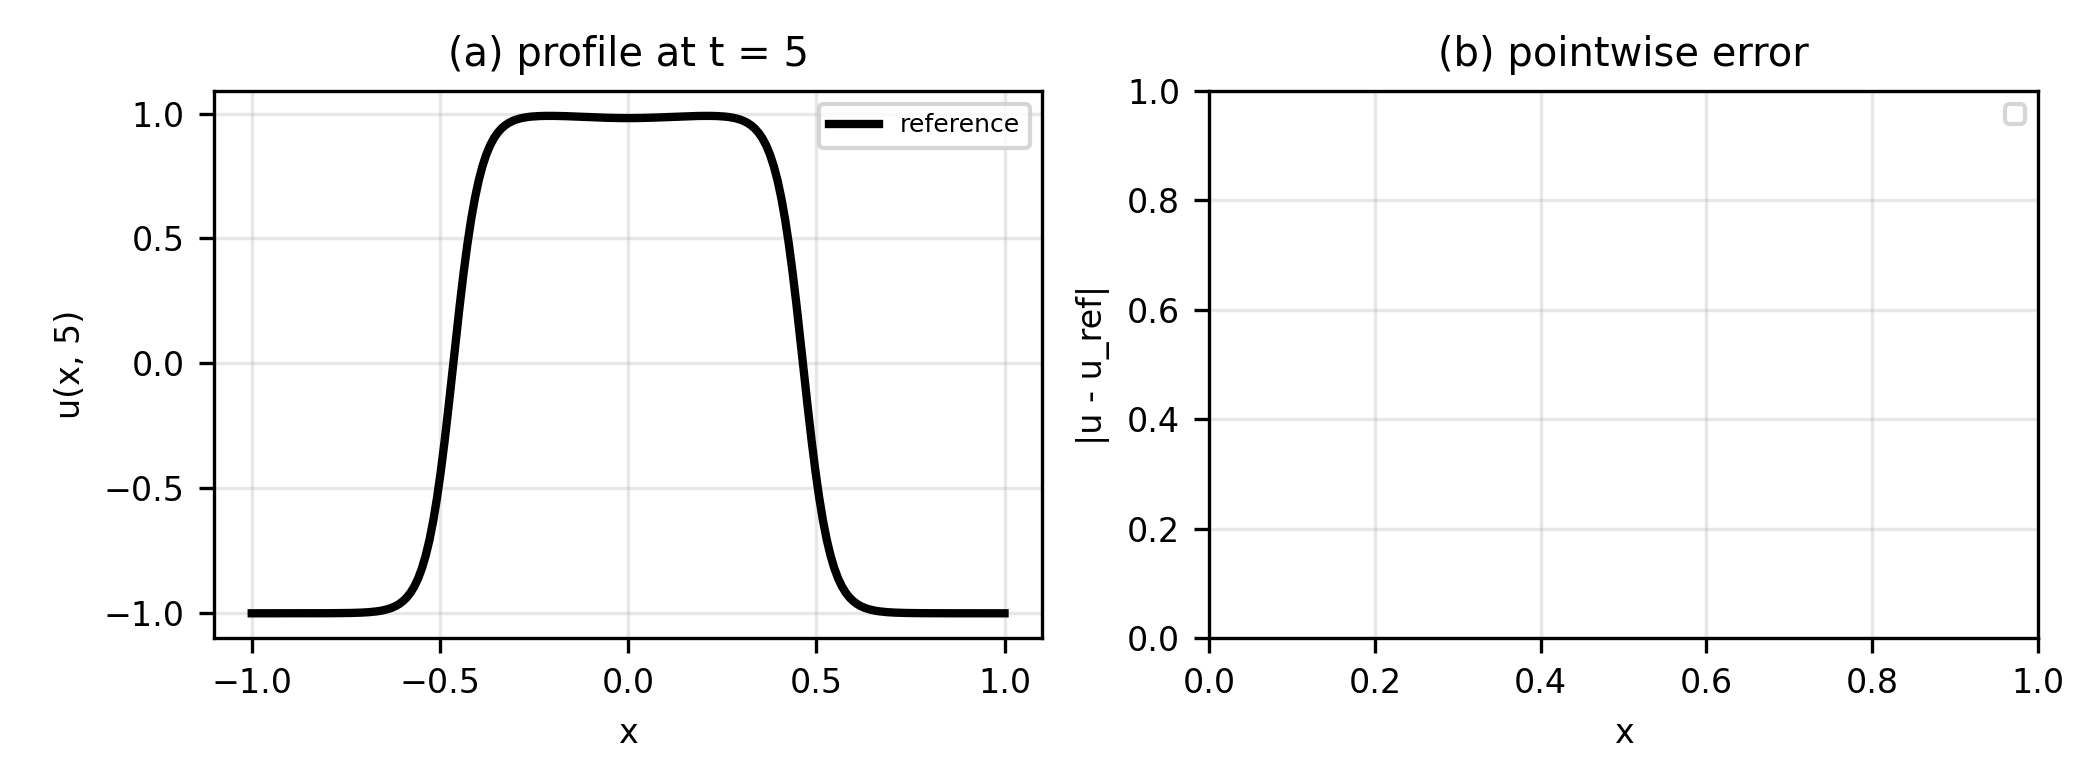
\includegraphics[width=\textwidth]{figures_r1/fig_b3.png}
\caption{\rev{B3 ($\varepsilon=0.05$, $T=5$, seed 42): certified reference and trained networks at $t=1$, $3$ and $5$.}\label{fig:b3}}
\end{figure}


\subsection{Mode Number: The Large Degradation Reported Previously Was a Boundary-Penalty Artifact}\label{sec:results-k}

\rev{The first version reported that the accuracy of the Spectral-PINN \emph{degrades} as the number of Chebyshev modes $K$ grows, and interpreted this as an optimization bottleneck of the coefficient parameterization. The large degradation was an artifact of the boundary treatment. In that code the Neumann penalty acted on $u_x(\pm1,t)/K^2$ and was then squared, so its effective weight on $u_x(\pm1)^2$ was $\lambda_{\rm BC}K^{-4}$ and vanished as $K$ grew: the trained $K=64$ networks of the as-submitted variant have wall slopes $|u_x(\pm1)|$ up to \N{kk.soft64.wall} instead of zero, and the $K=128$ network up to \N{kk.soft128.wall} (Table~\ref{tab:K}). With the exact Neumann basis the $L^2$ error at $K=64$ is \N{kk.hard64.l2} (five seeds), against \N{kk.soft64.l2} for the as-submitted variant (a factor \N{kk.ratio_soft_hard64}); at $K=128$ the numbers are \N{kk.hard128.l2} and \N{kk.soft128.l2} (Figure~\ref{fig:K}).}

\rev{Rescaling the soft penalty to unit effective weight ($\lambda_{\rm BC}=K^4$) does \emph{not} repair it; it makes it worse (\N{kk.fix64.l2} at $K=64$, $\max|u|$ up to \N{kk.fix64.maxu}). The rescaled penalty $(\sum_kk^2c_k)^2$ has a curvature of order $K^5/5$ in coefficient space ($2\times10^8$ at $K=64$), orders of magnitude above that of the other loss terms, and with this conditioning the optimizer no longer reduces the PDE residual: its time-RMS norm is \N{kk.fix64.rms}, against \N{kk.hard64.rms} for the exact basis, while the wall slope is still \N{kk.fix64.wall}. A soft Neumann penalty thus fails at large $K$ in both directions, too weak when scaled down with the mode number and ill-conditioned when not, and the exact basis removes the dilemma. The collocation grid has a secondary effect: Gauss--Lobatto instead of equispaced collocation improves the soft variant at $K=64$ by a factor \N{kk.cgl_soft_gain} (seed 42: \N{kk.soft_uniform64_s42} to \N{kk.soft_cgl64}) but leaves it far from the hard variant, and with the exact basis the grid matters little (\N{kk.hard_uniform64} equispaced, \N{kk.hard_cgl64_s42} Gauss--Lobatto, seed 42).}

\rev{With the revised variant and the default budget a smaller trend remains: the error grows from \N{kk.hard32.l2} at $K=32$ by a factor \N{kk.ratio64_32} to $K=64$ and by a further factor \N{kk.ratio128_64} to $K=128$. This is a matter of optimization, not of representation (the best polynomials of degree 64 and 128 approximate the solution to \N{floor.b1.K64} and \N{floor.b1.K128}), and it responds to the budget: doubling the epochs reduces the $K=64$ error of seed 42 from \N{kk.hard_cgl64_s42} to \N{kk.kh_K64_x2.l2}, below the floor of $K=32$ (\N{floor.b1.K32.neumann}), and an L-BFGS stage after Adam gives \N{b1.lb_hard_K64.l2} (two seeds). At $K=128$ twice the budget gives \N{kk.kh_K128_x2.l2} (default: \N{kk.hard128_s42}); at $K=256$ the default budget gives \N{kk.kh_K256_x1.l2} (seed 42), against $1.5$ for the as-submitted network in the first version. A larger $K$ thus needs a larger budget, but the errors of order one of the first version do not occur.}

% generated by make_tex_r1.py -- do not edit
\begin{table}[H]
\begin{adjustwidth}{-\extralength}{0cm}
\tablesize{\footnotesize}
\caption{$L^2$ error at $t=1$ on B1 versus the mode number $K$ for the four combinations of boundary treatment (soft penalty / exact Neumann basis) and collocation grid (equispaced / Gauss--Lobatto, CGL); mean over the number of seeds in parentheses. ``As submitted'' = soft penalty with effective weight $K^{-4}$, equispaced grid; ``$\lambda_{\rm BC}=K^4$'' = the same with the penalty rescaled to unit effective weight; ``Revised'' = exact Neumann basis, CGL grid. The last column is the largest wall slope of the as-submitted networks (zero for the exact basis by construction).\label{tab:K}}
\newcolumntype{C}{>{\centering\arraybackslash}X}
\begin{tabularx}{\fulllength}{cCCCCCc}
\toprule
\ensuremath{\boldsymbol{K}} & \textbf{As submitted} & \ensuremath{\boldsymbol{\lambda_{\rm BC}=K^4}} & \textbf{Soft, CGL} & \textbf{Hard, equisp.} & \textbf{Revised} & \ensuremath{\boldsymbol{\max|u_x(\pm1)|}}\\
\midrule
32 & \ensuremath{1.27\times10^{-3}} (5) & \ensuremath{3.54\times10^{-1}} (3) & \ensuremath{9.33\times10^{-4}} (1) & \ensuremath{9.20\times10^{-4}} (1) & \ensuremath{8.29\times10^{-4}} (5) & 1.1\\
64 & \ensuremath{9.71\times10^{-2}} (5) & \ensuremath{3.98\times10^{-1}} (3) & \ensuremath{1.52\times10^{-2}} (1) & \ensuremath{2.07\times10^{-3}} (1) & \ensuremath{1.46\times10^{-3}} (5) & 6.7\\
128 & \ensuremath{3.26\times10^{-1}} (1) & \ensuremath{1.27} (1) & --- & --- & \ensuremath{6.68\times10^{-3}} (3) & 480\\
256 & --- & --- & --- & --- & \ensuremath{3.48\times10^{-2}} (1) & ---\\
\midrule
\multicolumn{7}{l}{\emph{Revised variant, seed 42, larger training budget}}\\
64 & \multicolumn{4}{l}{$2\times$ epochs (12\,000 + 2000 warm-up)} & \ensuremath{2.24\times10^{-4}} (default: \ensuremath{1.70\times10^{-3}}) & ---\\
128 & \multicolumn{4}{l}{$2\times$ epochs (12\,000 + 2000 warm-up)} & \ensuremath{1.46\times10^{-3}} (default: \ensuremath{5.29\times10^{-3}}) & ---\\
\bottomrule
\end{tabularx}
\end{adjustwidth}
\end{table}


\begin{figure}[H]
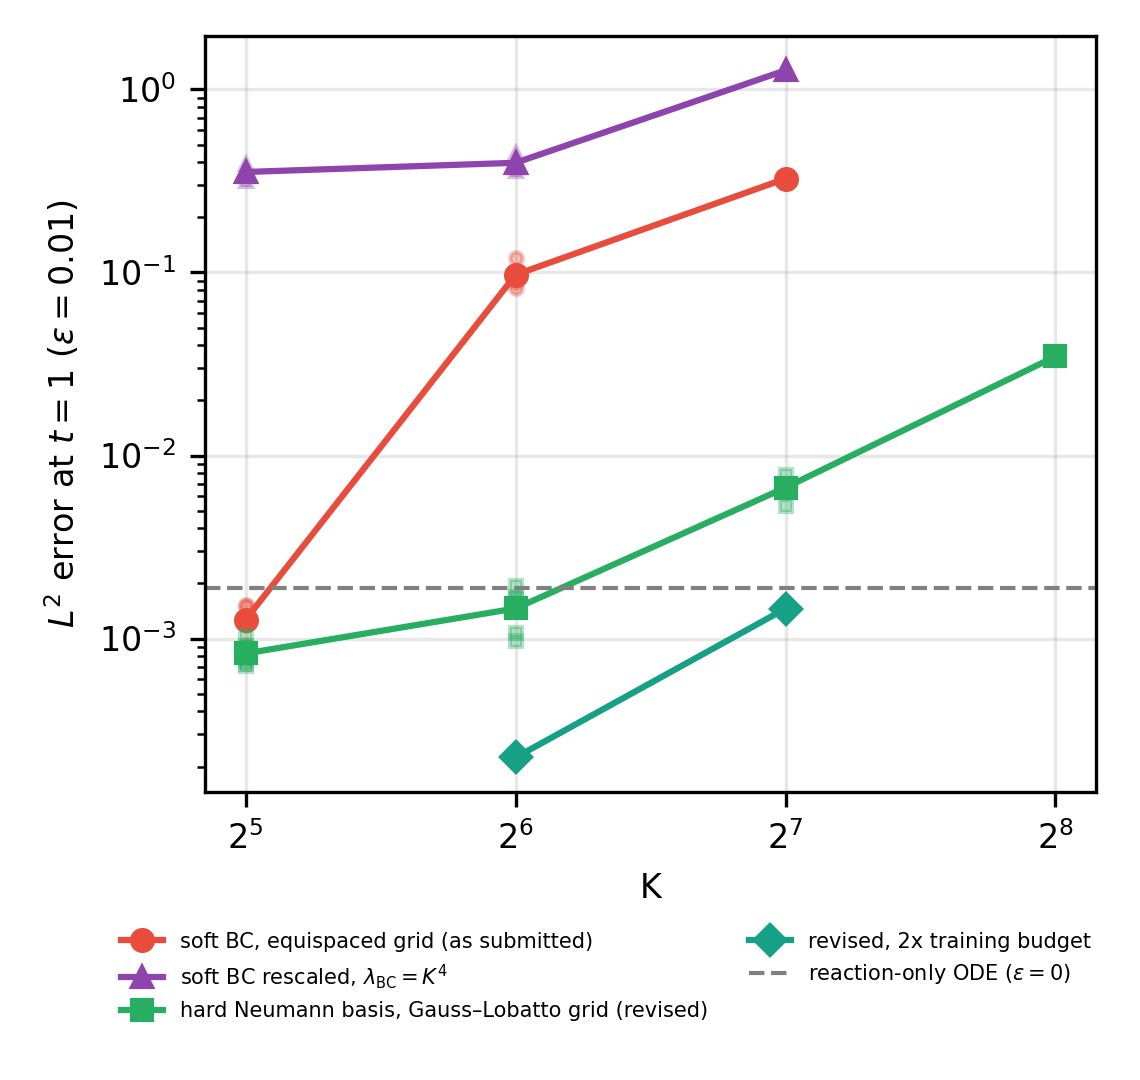
\includegraphics[width=8.5cm]{figures_r1/fig_K.png}
\caption{\rev{$L^2$ error at $t=1$ versus the mode number $K$ (B1; small symbols: individual seeds, large: mean): as-submitted soft penalty with effective weight $K^{-4}$, the same penalty rescaled to unit weight ($\lambda_{\rm BC}=K^4$), the revised Spectral-PINN (exact Neumann basis, Gauss--Lobatto collocation) at the default and at twice the default budget. The dashed line is the error of the reaction-only model.}\label{fig:K}}
\end{figure}


\subsection{Energy Penalty: Weight, Regimes and the Coinciding Energy Curves}\label{sec:results-energy}

\rev{The weight of the energy penalty in all penalized runs of the first version was $\lambda_E=50$ (it was not reported there). In B1, every Spectral-PINN trained for the forward problem---\N{en.n_runs} networks with and without the penalty, including the inaccurate ones of Section~\ref{sec:results-k} (errors up to \N{en.max_l2}) and those of the poor-trajectory regimes below---decreases its energy on every interval of the grids with spacing $0.02$, $0.002$ and $2\times10^{-4}$; the vanilla PINNs of B1 (grid $0.02$ only) have \N{en.van_viol} increases in \N{mbp.n_van} runs. For the revised $K=32$ network the energy decreases by at least \N{en.min_step} per interval of length $0.02$, whereas the penalty changes the energy trajectory by at most \N{en.max_diff} (same seed with and without it), which is why the two curves of Figure~\ref{fig:energy}(a) coincide: in this regime the penalty has no visible effect, and the zero violations of the first version cannot be attributed to it. The penalty term is positive in \N{en.nonzero} training epochs of the five runs with $\lambda_E=50$. Table~\ref{tab:energy} varies $\lambda_E$ from $0$ to $5000$: the mean error lies between \N{en.lam.min} and \N{en.lam.max} for all six weights (seed-to-seed SD at $\lambda_E=0$: \N{en.lam.sd}), no network has an energy increase, and the penalty is nonzero in at most \N{en.lam.max_nonzero} epoch per run (largest weighted value \N{en.lam.maxpen}, at $\lambda_E=5000$).}

\rev{We also looked for regimes in which the trajectory is poor: a run cut to \N{reg.short_epochs} epochs, no warm-up, a ten times smaller learning rate with 1500 epochs, and $K=64$ with the as-submitted soft penalty (Table~\ref{tab:energy}, lower part). In the truncated and slow runs the errors are large (\N{reg.short.E0} and \N{reg.pde0.E0}), but the energy is again monotone without the penalty, the penalty is active in at most \N{reg.pde0.E50.maxnz} epochs per run, and the errors with it (\N{reg.short.E50}, \N{reg.pde0.E50}) agree with those without it. For the as-submitted $K=64$ network the penalty is active in \N{reg.soft64.nz} epochs per run and changes the error by less than its seed-to-seed scatter (\N{reg.soft64.E50} against \N{reg.soft64.E0}, same seeds; slightly lower with the penalty for each of the three seeds). The only regime with a substantial effect is training without warm-up: the untrained initial trajectory has increasing energy, the penalty is active in up to \N{reg.nowarm.E50.maxnz} epochs per run with weighted values up to \N{reg.nowarm.E50.maxpen}, and the result is \emph{worse} (\N{reg.nowarm.E50} against \N{reg.nowarm.E0}; larger for all three seeds, by factors of \N{reg.nowarm.factors}). In none of the \N{reg.n_runs} runs of these regimes does the final network have an energy increase. Monotone energy is therefore not a diagnostic of accuracy for this problem: it is satisfied by networks whose error is of order one.}

% generated by make_tex_r1.py -- do not edit
\begin{table}[H]
\begin{adjustwidth}{-\extralength}{0cm}
\tablesize{\footnotesize}
\caption{Energy penalty: accuracy at $t=1$ (B1), number of energy increases of the trained trajectory on grids of spacing $0.02$, $0.002$ and $2\times10^{-4}$ (total over the seeds), number of training epochs in which the penalty was nonzero (summed over the seeds), and the largest value of the weighted penalty $\lambda_E\mathcal L_E$ during training (``---'': $\lambda_E=0$, for which $\mathcal L_E$ is not evaluated during training).\label{tab:energy}}
\newcolumntype{C}{>{\centering\arraybackslash}X}
\begin{tabularx}{\fulllength}{p{5.3cm}cCCcc}
\toprule
\textbf{Configuration} & \ensuremath{\boldsymbol{n}} & \ensuremath{\boldsymbol{\|e\|_{L^2}}} & \textbf{E incr.}~\ensuremath{\boldsymbol{0.02/0.002/0.0002}} & \textbf{Epochs with} \ensuremath{\boldsymbol{\mathcal L_E>0}} & \ensuremath{\boldsymbol{\max\lambda_E\mathcal L_E}}\\
\midrule
\multicolumn{6}{l}{\emph{B1, revised $K=32$: penalty weight}}\\
$\lambda_E=0$ & 5 & \ensuremath{(8.29\pm1.43)\times10^{-4}} & 0/0/0 & --- & ---\\
$\lambda_E=1$ & 5 & \ensuremath{(8.29\pm1.43)\times10^{-4}} & 0/0/0 & 5 & \ensuremath{4.7\times10^{-7}}\\
$\lambda_E=10$ & 5 & \ensuremath{(8.30\pm1.43)\times10^{-4}} & 0/0/0 & 5 & \ensuremath{4.7\times10^{-6}}\\
$\lambda_E=50$ & 5 & \ensuremath{(8.29\pm1.45)\times10^{-4}} & 0/0/0 & 5 & \ensuremath{2.3\times10^{-5}}\\
$\lambda_E=500$ & 5 & \ensuremath{(8.23\pm1.41)\times10^{-4}} & 0/0/0 & 5 & \ensuremath{2.3\times10^{-4}}\\
$\lambda_E=5000$ & 5 & \ensuremath{(8.30\pm1.29)\times10^{-4}} & 0/0/0 & 5 & \ensuremath{2.3\times10^{-3}}\\
\midrule
\multicolumn{6}{l}{\emph{Regimes with a poor trajectory ($K=32$ revised unless stated; 3 seeds)}}\\
300 epochs (100 warm-up), $\lambda_E=0$ & 3 & \ensuremath{(7.60\pm1.54)\times10^{-2}} & 0/0/0 & --- & ---\\
300 epochs (100 warm-up), $\lambda_E=50$ & 3 & \ensuremath{(7.60\pm1.55)\times10^{-2}} & 0/0/0 & 2 & \ensuremath{5.2\times10^{-5}}\\
no warm-up, $\lambda_E=0$ & 3 & \ensuremath{(6.46\pm6.88)\times10^{-3}} & 0/0/0 & --- & ---\\
no warm-up, $\lambda_E=50$ & 3 & \ensuremath{(4.09\pm3.32)\times10^{-2}} & 0/0/0 & 46 & \ensuremath{3.3\times10^{1}}\\
1500 epochs, learning rate $10^{-4}$, $\lambda_E=0$ & 3 & \ensuremath{(6.92\pm1.40)\times10^{-2}} & 0/0/0 & --- & ---\\
1500 epochs, learning rate $10^{-4}$, $\lambda_E=50$ & 3 & \ensuremath{(6.93\pm1.41)\times10^{-2}} & 0/0/0 & 4 & \ensuremath{2.3\times10^{-5}}\\
$K=64$ as submitted, $\lambda_E=0$ & 3 & \ensuremath{(9.94\pm1.90)\times10^{-2}} & 0/0/0 & --- & ---\\
$K=64$ as submitted, $\lambda_E=50$ & 3 & \ensuremath{(9.49\pm2.15)\times10^{-2}} & 0/0/0 & 59 & \ensuremath{6.8\times10^{-2}}\\
\bottomrule
\end{tabularx}
\end{adjustwidth}
\end{table}


\begin{figure}[H]
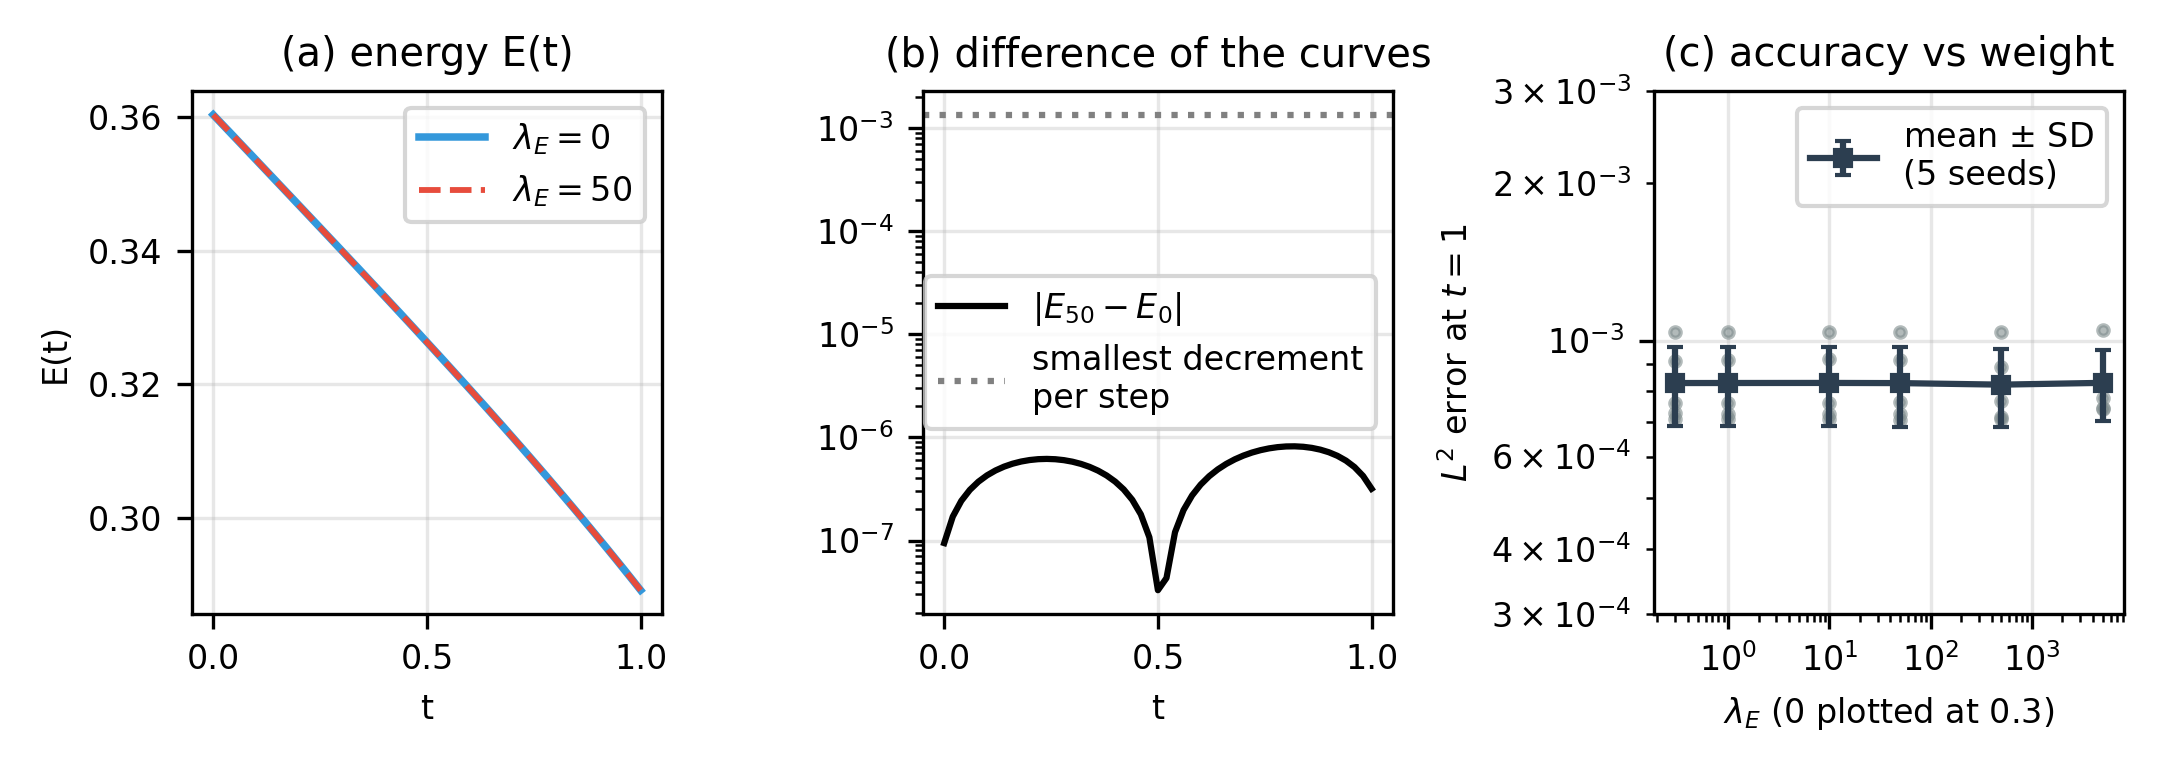
\includegraphics[width=\textwidth]{figures_r1/fig_energy.png}
\caption{\rev{Energy of the trained trajectory (B1, revised $K=32$, seed 42) with and without the energy penalty: (a) $E(t)$; (b) the absolute difference of the two curves compared with the smallest decrement of $E$ per grid interval; (c) mean $L^2$ error versus $\lambda_E$ (five seeds).}\label{fig:energy}}
\end{figure}


\subsection{Maximum Bound Principle and the A-Posteriori Energy Balance}\label{sec:results-balance}

\rev{\emph{Maximum bound.} The exact solution satisfies $|u|\le1$ (the certified reference of B1 has $\max|u|=\N{mbp.ref_max_t1}$ at $t=1$), but decreasing energy does not imply this~\cite{ref_Du2021b,ref_He2019}. We computed $\max_{x,t}|u_\theta|$ for every one-dimensional network trained on the forward problem (Table~\ref{tab:forward} gives the largest value per configuration). All \N{mbp.n_hard} revised Spectral-PINNs of B1 outside the poor-trajectory regimes exceed the bound slightly, by at most \N{mbp.excess} (largest value \N{mbp.max_hard}), and so do the \N{mbp.n_hard_reg} revised networks of those regimes, by up to \N{mbp.excess_reg} (largest value \N{mbp.max_hard_reg}); \N{mbp.n_van_over} of the \N{mbp.n_van} vanilla PINNs of B1 exceed it as well, by up to \N{mbp.van_excess}. These excesses are of the order of the approximation error, but the bound is \emph{not} guaranteed, and the inaccurate networks of Section~\ref{sec:results-k} violate it substantially ($\max|u|$ up to \N{kk.fix64.maxu} for the rescaled soft penalty and \N{kk.soft128.maxu} for the as-submitted network with $K=128$) although their energy decreases monotonically. A guaranteed bound would need an additional mechanism such as a limiter~\cite{ref_Geng2025}; we do not attempt one.}

\rev{\emph{Energy balance.} For every Spectral-PINN trained for the forward problem we evaluated both sides of the identity~\eqref{eq:balance-main} and the bound~\eqref{eq:balance-int} (Table~\ref{tab:balance}). The identity holds to round-off (largest relative deviation \N{bal.id_err} over all \N{bal.n} networks), which checks the code against Theorem~\ref{thm:balance}. The time-integrated residual $\frac12\int_0^T\|r\|^2\,dt$ of the revised $K=32$ networks (B1) is \N{bal.int_r_hard} on average and at most \N{bal.int_r_hard_max} over the five seeds, against an energy decrease $E(0)-E(T)=\N{bal.dE_hard}$: the energy of none of these networks can increase between any two times by more than \N{bal.int_r_hard_max}, a fraction \N{bal.frac_hard_max} of its decrease, and it is $\|u_t\|^2$ rather than the residual that drives the decay. For the as-submitted soft variant at $K=64$ the residual term is \N{bal.int_r_soft64} and the boundary defect adds \N{bal.int_b_soft}. Figure~\ref{fig:balance}(a) compares both sides of the identity along a trained trajectory, and Figure~\ref{fig:balance}(b) shows the residual of trained networks.}

% generated by make_tex_r1.py -- do not edit
\begin{table}[H]
\begin{adjustwidth}{-\extralength}{0cm}
\tablesize{\footnotesize}
\caption{A-posteriori energy balance~\eqref{eq:balance-int} of the trained networks (means over the seeds): time-RMS of the residual norm, the integrated residual term, the time integral of the absolute value of the boundary term $\beta=\varepsilon^2[u_xu_t]_{-1}^{1}$, the actual energy decrease, the largest wall slope, and the largest relative deviation between $dE/dt$, evaluated as $\int(\varepsilon^2u_xu_{xt}+f(u)u_t)\,dx$ with $\dot{\mathbf c}$ from automatic differentiation, and the right-hand side of~\eqref{eq:balance-main} over 201 times.\label{tab:balance}}
\newcolumntype{C}{>{\centering\arraybackslash}X}
\begin{tabularx}{\fulllength}{p{4.4cm}cCCCCCc}
\toprule
\textbf{Configuration} & \ensuremath{\boldsymbol{n}} & \ensuremath{\boldsymbol{(\frac1T\int\|r\|^2)^{1/2}}} & \ensuremath{\boldsymbol{\frac12\int\|r\|^2}} & \ensuremath{\boldsymbol{\int|\beta|}} & \ensuremath{\boldsymbol{E(0)-E(T)}} & \ensuremath{\boldsymbol{\max|u_x(\pm1)|}} & \textbf{Identity}\\
\midrule
B1 revised $K=32$ & 5 & \ensuremath{5.0\times10^{-3}} & \ensuremath{1.3\times10^{-5}} & \ensuremath{3.7\times10^{-22}} & \ensuremath{7.12\times10^{-2}} & \ensuremath{3.6\times10^{-15}} & \ensuremath{3\times10^{-16}}\\
B1 revised $K=32$, $\lambda_E=50$ & 5 & \ensuremath{5.0\times10^{-3}} & \ensuremath{1.3\times10^{-5}} & \ensuremath{4.1\times10^{-22}} & \ensuremath{7.12\times10^{-2}} & \ensuremath{3.6\times10^{-15}} & \ensuremath{3\times10^{-16}}\\
B1 revised $K=64$ & 5 & \ensuremath{6.4\times10^{-3}} & \ensuremath{2.1\times10^{-5}} & \ensuremath{4.0\times10^{-22}} & \ensuremath{7.11\times10^{-2}} & \ensuremath{4.4\times10^{-15}} & \ensuremath{3\times10^{-16}}\\
B1 revised $K=128$ & 3 & \ensuremath{1.1\times10^{-2}} & \ensuremath{6.0\times10^{-5}} & \ensuremath{1.9\times10^{-21}} & \ensuremath{6.99\times10^{-2}} & \ensuremath{7.1\times10^{-15}} & \ensuremath{3\times10^{-16}}\\
B1 as submitted $K=32$ & 5 & \ensuremath{8.0\times10^{-3}} & \ensuremath{3.2\times10^{-5}} & \ensuremath{3.0\times10^{-7}} & \ensuremath{7.10\times10^{-2}} & \ensuremath{1.1} & \ensuremath{5\times10^{-16}}\\
B1 as submitted $K=64$ & 5 & \ensuremath{3.0\times10^{-2}} & \ensuremath{4.6\times10^{-4}} & \ensuremath{4.7\times10^{-6}} & \ensuremath{5.85\times10^{-2}} & \ensuremath{6.7} & \ensuremath{4\times10^{-16}}\\
B1 soft, $\lambda_{\rm BC}=K^4$, $K=64$ & 3 & \ensuremath{3.0\times10^{-1}} & \ensuremath{4.6\times10^{-2}} & \ensuremath{1.7\times10^{-6}} & \ensuremath{3.81\times10^{-2}} & \ensuremath{1.2} & \ensuremath{2\times10^{-15}}\\
B2 revised $K=32$ & 5 & \ensuremath{1.5\times10^{-2}} & \ensuremath{1.2\times10^{-4}} & \ensuremath{2.6\times10^{-19}} & \ensuremath{5.37\times10^{-2}} & \ensuremath{2.7\times10^{-15}} & \ensuremath{6\times10^{-16}}\\
B3 revised $K=64$ ($T=5$) & 2 & \ensuremath{3.6\times10^{-2}} & \ensuremath{3.2\times10^{-3}} & \ensuremath{2.3\times10^{-19}} & \ensuremath{1.64\times10^{-1}} & \ensuremath{1.7\times10^{-14}} & \ensuremath{6\times10^{-16}}\\
\bottomrule
\end{tabularx}
\end{adjustwidth}
\end{table}


\begin{figure}[H]
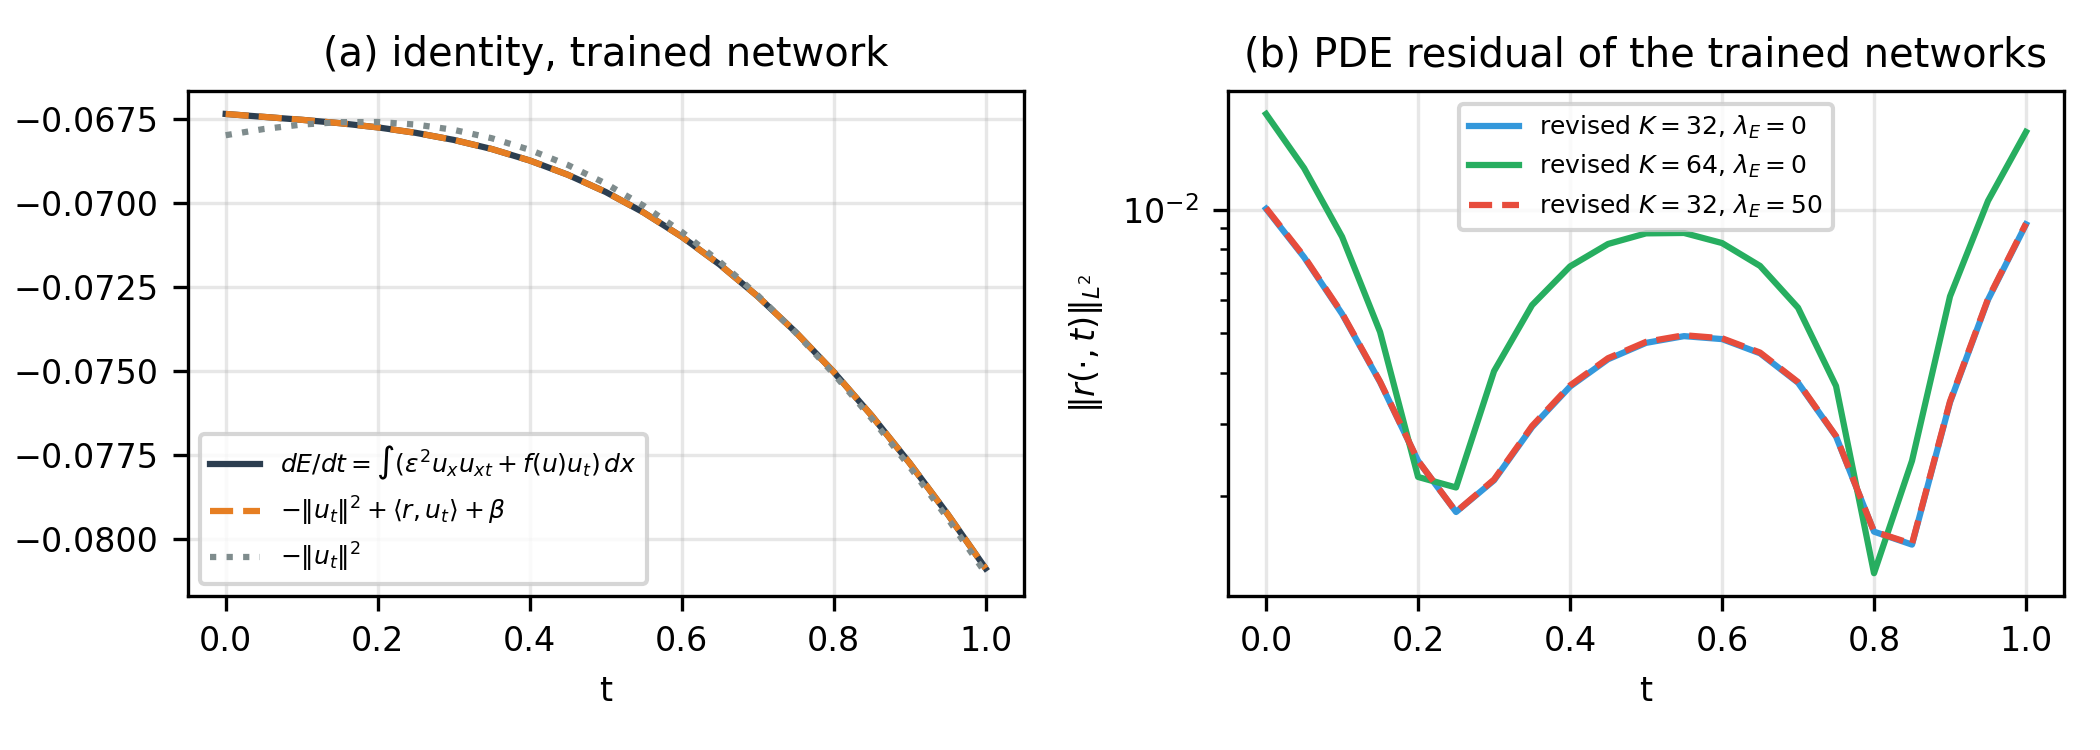
\includegraphics[width=\textwidth]{figures_r1/fig_balance.png}
\caption{\rev{(a) The two sides of the energy identity~\eqref{eq:balance-main} along the trained trajectory (B1, revised $K=32$, $\lambda_E=50$, seed 42): they coincide to round-off. (b) $L^2$ norm of the PDE residual versus time for the revised networks with $K=32$ without and with the energy penalty ($\lambda_E=0$, solid; $\lambda_E=50$, dashed; the curves nearly coincide) and with $K=64$ (B1, seed 42).}\label{fig:balance}}
\end{figure}


\subsection{\texorpdfstring{\protect\textcolor{black}{Inverse Problem}}{Inverse Problem}}\label{sec:results-inverse}

\rev{\emph{Joint Adam depends on the starting value.} The first version reported a ``robust $\sim38\%$ overestimation bias'' of the recovered $\varepsilon$ and attributed it to the loss weighting, the warm-up or the observation design, without an ablation. It is the footprint of the starting value and of the optimizer. With the joint-Adam procedure of Section~\ref{sec:inverse} the recovered value is $\hat\varepsilon\approx\N{inv.ratio_mean}\,\varepsilon_{\rm init}$ (range \N{inv.ratio_range} over \N{inv.n_sweep} runs) for every $\varepsilon_{\rm init}\in\{0.5,1,1.5,2,4\}\,\varepsilon_{\rm true}$, for $\varepsilon_{\rm true}\in\{0.05,0.1\}$ and for both the as-submitted and the revised network (Figure~\ref{fig:inverse}(a), Table~\ref{tab:inverse1}); all runs of the first version that produced the $38\%$ had started from $\varepsilon_{\rm init}=2\varepsilon_{\rm true}$, and $0.7\times2=1.4$ is the ``bias''. Most of the displacement of $\log\varepsilon$ happens at the beginning of the joint phase (median \N{inv.frac200}, at least \N{inv.frac200_min}, of the total within the first 200 of 4000 epochs), and its size is set by the learning rate of $\log\varepsilon$: the displacement $|\log(\hat\varepsilon/\varepsilon_{\rm init})|$ is \N{inv.ab.mult1.disp}, \N{inv.ab.base.disp} and \N{inv.ab.mult100.disp} for learning-rate multipliers $1$, $10$ (default) and $100$ (Table~\ref{tab:inverse2}). The data enter only weakly: with 10, 40 or 160 observation points, 5 or 20 observation times, $K=16$, $32$ or $64$ and $\lambda_{\rm PDE}=5$, $50$ or $500$ the estimate lies in the range \N{inv.ab.design_range}$\,\varepsilon_{\rm true}$; a thousand times larger data weight moves it to \N{inv.ab.ld2000.rt}$\,\varepsilon_{\rm true}$, and four times more epochs to \N{inv.ab.ep16000.rt}$\,\varepsilon_{\rm true}$. Started from the true value, the estimate first moves away from it, to about $0.7\,\varepsilon_{\rm true}$ within 200 epochs; with the large data weight the data pull it back to \N{inv.ab.ld2000_i1.rt}$\,\varepsilon_{\rm true}$, with the default one it ends at \N{inv.i1.rt}$\,\varepsilon_{\rm true}$. The relative errors reported in the first version for the noise experiments at $\varepsilon_{\rm true}=0.01$ ($40.2$, $40.2$ and $40.0\%$ for $\sigma=0$, $0.01$ and $0.05$) and for a single run at $\varepsilon_{\rm true}=0.05$ ($14.7\%$) came from a script whose settings differed from those stated and whose output was not archived; they are withdrawn.}

\rev{\emph{An estimator that does not depend on the start.} Variable projection (Section~\ref{sec:inverse}), combined with a data-fitting phase and a large data weight, recovers $\varepsilon$ from noise-free data with relative errors of \N{inv.vp_err_005} ($\varepsilon_{\rm true}=0.05$) and \N{inv.vp_err_01} ($0.1$) at $\lambda_{\rm data}=2000$ (Figure~\ref{fig:inverse}(b), Table~\ref{tab:inverse2}). It needs a large data weight and enough observation points: with $\lambda_{\rm data}=20$ the errors are \N{inv.vp.e0.05.ld20} and \N{inv.vp.e0.1.ld20}, and with only 10 observation points the error is \N{inv.vp.nx10}; with $K=64$ the least-squares value of $\varepsilon^2$ collapsed to the lower bound $10^{-8}$ of its admissible range during training. \emph{It is not robust to noise} (Table~\ref{tab:inverse3}, Figure~\ref{fig:inverse}(c)): with $\sigma=0.01$ it underestimates $\varepsilon$ by \N{inv.vpn.e0.05.n0.01} ($\varepsilon_{\rm true}=0.05$) and \N{inv.vpn.e0.1.n0.01} ($0.1$) on average over five noise realizations, and with $\sigma=0.05$ it collapses toward $\varepsilon=0$ (largest estimate \N{inv.vpn.e0.1.n0.05.maxratio}$\,\varepsilon_{\rm true}$). A plausible mechanism, not investigated further, is that with a large data weight the network fits part of the noise, which increases $\|u_{xx}\|$ and decreases the least-squares value. The classical least-squares estimator (Section~\ref{sec:inverse}) has, on the same realizations, mean errors of \N{inv.cl5.e0.05.n0.01} and \N{inv.cl5.e0.1.n0.01} ($\sigma=0.01$) and \N{inv.cl5.e0.05.n0.05} and \N{inv.cl5.e0.1.n0.05} ($\sigma=0.05$), in line with the Cram\'er--Rao bound; in the noise-free case it recovers the true value to better than $10^{-3}\%$, since the data come from the same solver.}

% generated by make_tex_r1.py -- do not edit
\begin{table}[H]
\tablesize{\footnotesize}
\caption{Joint Adam (procedure of the first version): estimate $\hat\varepsilon/\varepsilon_{\rm true}$ for five starting values, noise-free data, seed 42. Last row: $\hat\varepsilon/\varepsilon_{\rm init}$, mean~$\pm$~SD over the five starting values.\label{tab:inverse1}}
\newcolumntype{C}{>{\centering\arraybackslash}X}
\begin{tabularx}{\textwidth}{cCCCC}
\toprule
\ensuremath{\boldsymbol{\varepsilon_{\rm init}/\varepsilon_{\rm true}}} & \multicolumn{2}{c}{$\boldsymbol{\varepsilon_{\rm true}=0.05}$} & \multicolumn{2}{c}{$\boldsymbol{\varepsilon_{\rm true}=0.1}$}\\
 & \textbf{as submitted} & \textbf{revised} & \textbf{as submitted} & \textbf{revised}\\
\midrule
0.50 & 0.361 & 0.307 & 0.357 & 0.342\\
1.0 & 0.713 & 0.679 & 0.717 & 0.685\\
1.5 & 1.08 & 1.10 & 1.08 & 1.01\\
2.0 & 1.43 & 1.37 & 1.43 & 1.37\\
4.0 & 2.87 & 2.73 & 2.87 & 2.81\\
\midrule
$\hat\varepsilon/\varepsilon_{\rm init}$ & \ensuremath{0.717\pm0.003} & \ensuremath{0.678\pm0.043} & \ensuremath{0.716\pm0.002} & \ensuremath{0.685\pm0.011}\\
\bottomrule
\end{tabularx}
\end{table}

\begin{table}[H]
\tablesize{\footnotesize}
\caption{Inverse problem, noise-free data: sensitivity of the joint-Adam estimate and of the variable-projection estimate to the settings (one run each, seed 42).\label{tab:inverse2}}
\newcolumntype{C}{>{\centering\arraybackslash}X}
\begin{tabularx}{\textwidth}{Xcccc}
\toprule
\textbf{Setting} & \ensuremath{\boldsymbol{\varepsilon_{\rm true}}} & \ensuremath{\boldsymbol{\hat\varepsilon/\varepsilon_{\rm true}}} & \ensuremath{\boldsymbol{\hat\varepsilon/\varepsilon_{\rm init}}} & \textbf{Data RMS misfit}\\
\midrule
\multicolumn{5}{l}{\emph{Joint Adam, revised network, $\varepsilon_{\rm init}=2\varepsilon_{\rm true}$}}\\
default ($\lambda_{\rm data}=2$, 40 points, 5 times, $K=32$) & 0.05 & 1.37 & 0.685 & \ensuremath{1.4\times10^{-2}}\\
$\lambda_{\rm data}=2000$ & 0.05 & 1.14 & 0.572 & \ensuremath{1.5\times10^{-3}}\\
$\lambda_{\rm data}=2000$, $\varepsilon_{\rm init}=\varepsilon_{\rm true}$ & 0.05 & 1.02 & 1.02 & \ensuremath{1.1\times10^{-3}}\\
10 observation points & 0.05 & 1.36 & 0.681 & \ensuremath{1.5\times10^{-2}}\\
160 observation points & 0.05 & 1.37 & 0.684 & \ensuremath{1.4\times10^{-2}}\\
20 observation times & 0.05 & 1.32 & 0.661 & \ensuremath{1.4\times10^{-2}}\\
$K=16$ & 0.05 & 1.32 & 0.662 & \ensuremath{1.2\times10^{-2}}\\
$K=64$ & 0.05 & 1.29 & 0.647 & \ensuremath{1.1\times10^{-2}}\\
$\lambda_{\rm PDE}=5$ & 0.05 & 1.30 & 0.652 & \ensuremath{5.6\times10^{-3}}\\
$\lambda_{\rm PDE}=500$ & 0.05 & 1.30 & 0.648 & \ensuremath{6.9\times10^{-2}}\\
learning-rate multiplier of $\log\varepsilon$: 1 (default 10) & 0.05 & 1.81 & 0.907 & \ensuremath{2.1\times10^{-2}}\\
learning-rate multiplier of $\log\varepsilon$: 100 & 0.05 & 0.168 & 0.0842 & \ensuremath{1.1\times10^{-2}}\\
16\,000 epochs (default 4000) & 0.05 & 0.705 & 0.352 & \ensuremath{4.0\times10^{-3}}\\
\midrule
\multicolumn{5}{l}{\emph{Variable projection (data-fit phase of 3000 epochs, $\lambda_{\rm data}$ as given), noise-free data}}\\
$\lambda_{\rm data}=20$ & 0.05 & 0.812 & --- & \ensuremath{2.7\times10^{-3}}\\
$\lambda_{\rm data}=200$ & 0.05 & 0.983 & --- & \ensuremath{9.2\times10^{-4}}\\
$\lambda_{\rm data}=2000$ & 0.05 & 1.01 & --- & \ensuremath{7.3\times10^{-4}}\\
$\lambda_{\rm data}=20\,000$ & 0.05 & 0.988 & --- & \ensuremath{9.5\times10^{-4}}\\
$\lambda_{\rm data}=20$ & 0.1 & 0.662 & --- & \ensuremath{1.2\times10^{-2}}\\
$\lambda_{\rm data}=200$ & 0.1 & 0.949 & --- & \ensuremath{3.0\times10^{-3}}\\
$\lambda_{\rm data}=2000$ & 0.1 & 0.997 & --- & \ensuremath{1.1\times10^{-3}}\\
$\lambda_{\rm data}=20\,000$ & 0.1 & 1.00 & --- & \ensuremath{1.0\times10^{-3}}\\
10 observation points ($\lambda_{\rm data}=2000$) & 0.05 & 0.318 & --- & \ensuremath{8.7\times10^{-4}}\\
160 observation points ($\lambda_{\rm data}=2000$) & 0.05 & 1.00 & --- & \ensuremath{7.6\times10^{-4}}\\
3 observation times ($\lambda_{\rm data}=2000$) & 0.05 & 1.04 & --- & \ensuremath{7.4\times10^{-4}}\\
20 observation times ($\lambda_{\rm data}=2000$) & 0.05 & 0.992 & --- & \ensuremath{8.5\times10^{-4}}\\
$\lambda_{\rm PDE}=5$ ($\lambda_{\rm data}=2000$) & 0.05 & 0.988 & --- & \ensuremath{9.4\times10^{-4}}\\
$\lambda_{\rm PDE}=500$ ($\lambda_{\rm data}=2000$) & 0.05 & 0.982 & --- & \ensuremath{9.5\times10^{-4}}\\
no data-fit phase ($\lambda_{\rm data}=2000$) & 0.05 & 1.02 & --- & \ensuremath{1.0\times10^{-3}}\\
$K=64$ ($\lambda_{\rm data}=2000$) & 0.05 & 0.00200 & --- & \ensuremath{1.6\times10^{-3}}\\
\bottomrule
\end{tabularx}
\end{table}

\begin{table}[H]
\begin{adjustwidth}{-\extralength}{0cm}
\tablesize{\footnotesize}
\caption{Inverse problem with noisy data: relative error $|\hat\varepsilon-\varepsilon_{\rm true}|/\varepsilon_{\rm true}$ of the variable-projection Spectral-PINN ($\lambda_{\rm data}=2000$; mean~$\pm$~SD over five noise realizations, one run for $\varepsilon_{\rm true}=0.01$ and for noise-free data) and of the classical least-squares estimator on the same five realizations (noise seeds 1--5; for $\varepsilon_{\rm true}=0.01$ the network was run only on the first of them with $\sigma=0.01$ and not at all with $\sigma=0.05$) and on 25 realizations (root-mean-square error); Fisher s.e.: Cram\'er--Rao standard error $\sigma/\|\partial u_{\rm obs}/\partial\log\varepsilon\|$ of $\log\hat\varepsilon$.\label{tab:inverse3}}
\newcolumntype{C}{>{\centering\arraybackslash}X}
\begin{tabularx}{\fulllength}{ccCCCC}
\toprule
\ensuremath{\boldsymbol{\varepsilon_{\rm true}}} & \ensuremath{\boldsymbol{\sigma}} & \textbf{Var. projection (5 real.)} & \textbf{Classical LS (same 5)} & \textbf{Classical LS (25), RMSE} & \textbf{Fisher s.e.}\\
\midrule
0.01 & 0 & \ensuremath{22}\% & \ensuremath{<10^{-3}}\% & --- & ---\\
0.01 & 0.01 & \ensuremath{90}\% & \ensuremath{53\pm44}\% & 41\% & 45\%\\
0.01 & 0.05 & --- & \ensuremath{79\pm35}\% & 100\% & 230\%\\
\midrule
0.05 & 0 & \ensuremath{0.62}\% & \ensuremath{<10^{-3}}\% & --- & ---\\
0.05 & 0.01 & \ensuremath{11\pm1.4}\% & \ensuremath{1.8\pm1.3}\% & 1.7\% & 2.0\%\\
0.05 & 0.05 & \ensuremath{99\pm1.3}\% & \ensuremath{9.5\pm7.0}\% & 8.4\% & 10\%\\
\midrule
0.1 & 0 & \ensuremath{0.33}\% & \ensuremath{<10^{-3}}\% & --- & ---\\
0.1 & 0.01 & \ensuremath{3.0\pm0.86}\% & \ensuremath{0.60\pm0.44}\% & 0.59\% & 0.68\%\\
0.1 & 0.05 & \ensuremath{96\pm4.5}\% & \ensuremath{3.0\pm2.2}\% & 2.9\% & 3.4\%\\
\bottomrule
\end{tabularx}
\end{adjustwidth}
\end{table}


\begin{figure}[H]
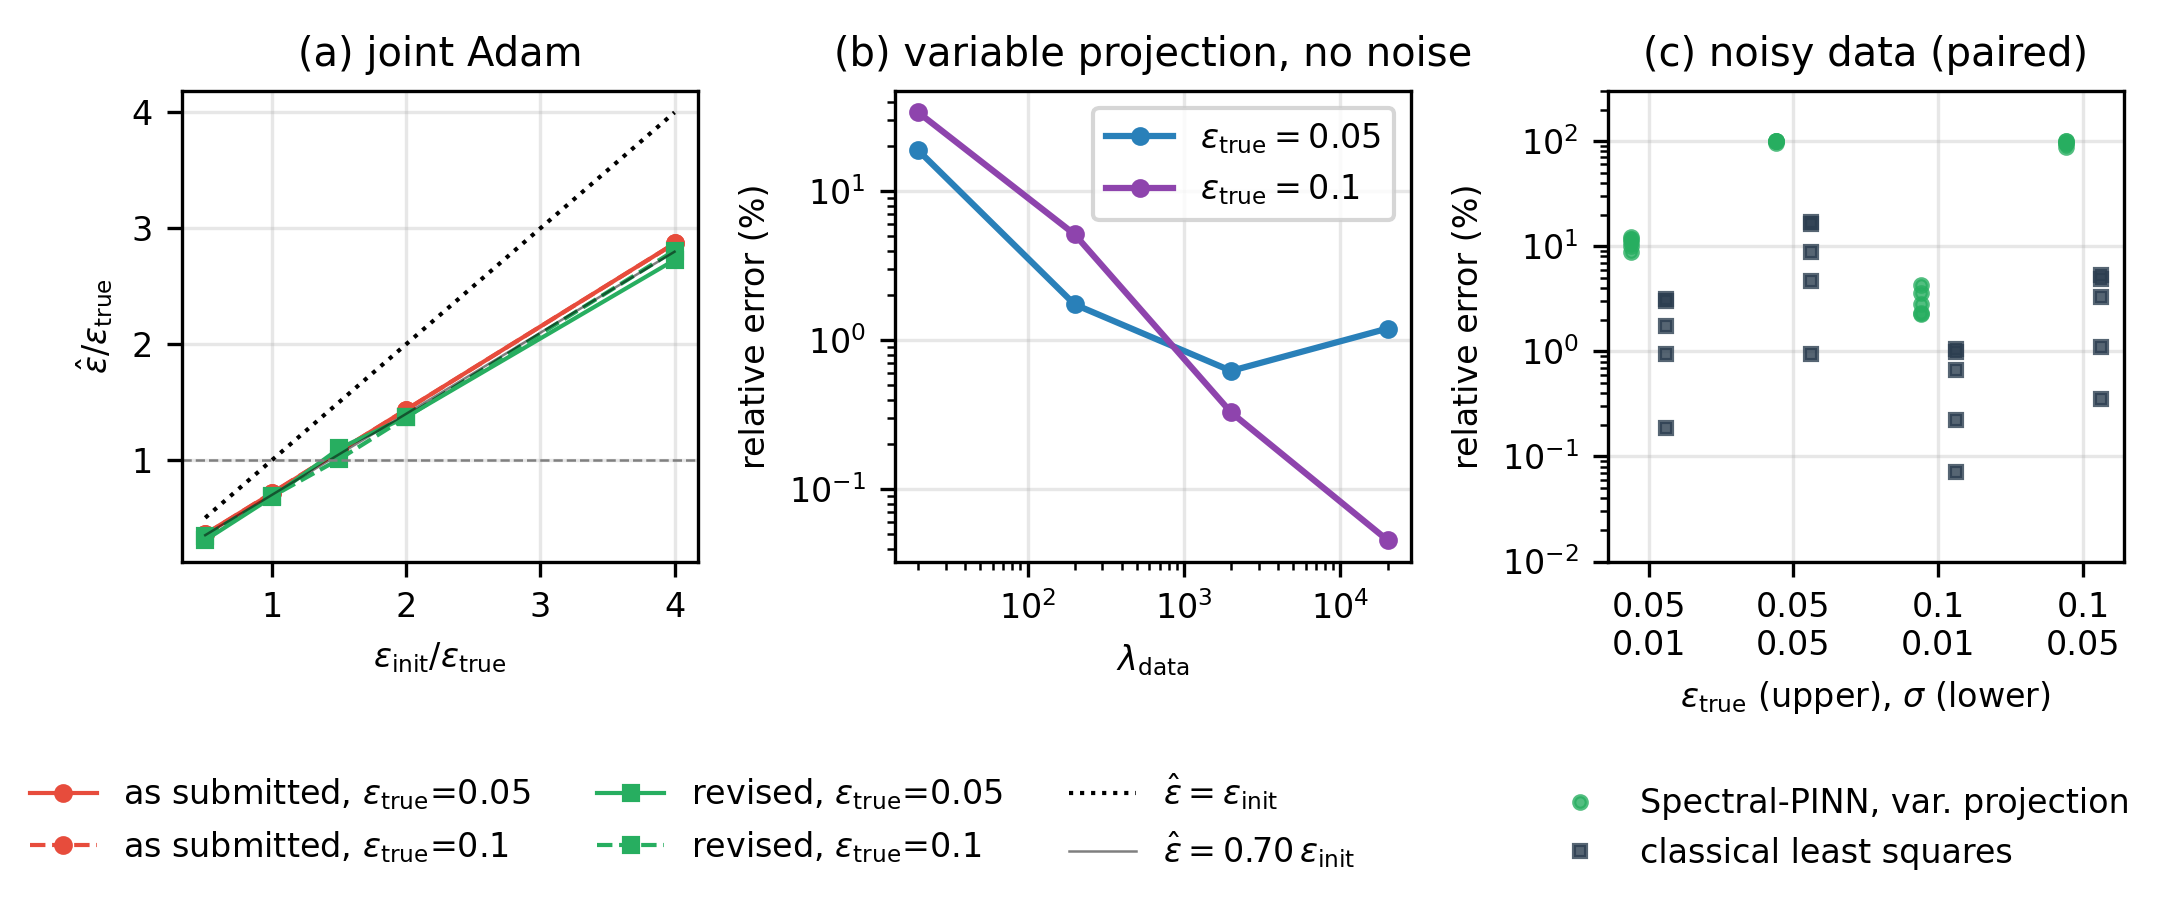
\includegraphics[width=\textwidth]{figures_r1/fig_inverse.png}
\caption{\rev{(a) Joint Adam: $\hat\varepsilon/\varepsilon_{\rm true}$ versus the starting value for the as-submitted and the revised network; the estimate follows $\approx0.7\,\varepsilon_{\rm init}$ (dotted: no change; dashed: the true value). (b) Variable projection: relative error versus the data weight, noise-free data. (c) Noisy data: relative errors of the variable-projection Spectral-PINN and of classical least squares on the same five noise realizations (horizontal axis: $\varepsilon_{\rm true}$, upper row, and $\sigma$, lower row).}\label{fig:inverse}}
\end{figure}

\rev{\emph{Identifiability.} The data constrain $\varepsilon$ only through the term $\varepsilon^2u_{xx}$, which is small on this benchmark. For our observation design (40 points, 5 times) the norm of the derivative of the data vector with respect to $\log\varepsilon$ is \N{ident.S001} at $\varepsilon=0.01$, \N{ident.S005} at $0.05$ and \N{ident.S01} at $0.1$. With noise $\sigma=0.01$ the Cram\'er--Rao standard error of $\log\hat\varepsilon$ is therefore \N{ident.se001} at $\varepsilon=0.01$ (\N{ident.se005} at $0.05$), and classical least squares indeed has a root-mean-square error of \N{ident.cl001} there (\N{ident.cl005} at $0.05$; \N{ident.n_rep} noise realizations). For $\varepsilon=0.01$ no unbiased estimator can recover $\varepsilon$ from such data to better than about \N{ident.se001}; the noise experiments at $\varepsilon=0.01$ of the first version were therefore not meaningful tests. (The variable-projection network has errors of \N{inv.vp001.n0} without and \N{inv.vp001.n0.01} with noise at $\varepsilon=0.01$.)}


\subsection{Two-Dimensional Symmetry Preservation}\label{sec:2d-results}

\rev{The two-dimensional results are unchanged from the first version (no Neumann condition is involved); the statements about them are corrected.} Table~\ref{tab:2d} gives the reflection-symmetry violation $S(t)$. The Fourier-Spectral-PINN stays at round-off, $S\in[\N{s2d.fmin},\N{s2d.fmax}]$ for $t\in[0,1]$ \rev{(one run; by the parity of the basis $S$ vanishes in exact arithmetic, and the value shown is the round-off of the evaluation grid, Appendix~\ref{app:sym}, not an effect of the training)}, while the vanilla PINN with the same periodic encoding has $S$ increasing monotonically in every one of the five seeds, by a factor of \N{s2d.growth} (seeds: \N{s2d.growth_range}) between $t=0$ and $t=1$. \rev{Larger mode counts and a sharper interface do not change this (Table~\ref{tab:stress-2d}): at $t=1$ the violation lies between \N{s2d.smin} and \N{s2d.smax} in all five configurations, at the level of round-off (the RMS asymmetry $\sqrt S$ is at most \N{s2d.rms_max}, about three times the machine epsilon). It is about three times larger for $\varepsilon=0.1$ than for $\varepsilon=0.3$, and doubling $M$ or the budget does not change it. (The first version gave the range as ``$10^{-31}$--$10^{-31.4}$'', inconsistent with its own table.)}

% generated by make_tex_r1.py -- do not edit
\begin{table}[H]
\tablesize{\footnotesize}
\caption{Reflection-symmetry violation $S(t)$ (Section~\ref{sec:2d}) of the Fourier-Spectral-PINN (one run; $M=8$, $\varepsilon=0.3$) and of a vanilla PINN with the same periodic input encoding (mean~$\pm$~SD over five seeds). Data of the first version, unchanged.\label{tab:2d}}
\newcolumntype{C}{>{\centering\arraybackslash}X}
\begin{tabularx}{\textwidth}{cCC}
\toprule
\ensuremath{\boldsymbol{t}} & \textbf{Fourier-Spectral-PINN} & \textbf{Vanilla PINN (5 seeds)}\\
\midrule
0.0 & \ensuremath{8.7\times10^{-32}} & \ensuremath{(4.12\pm1.13)\times10^{-5}}\\
0.2 & \ensuremath{9.4\times10^{-32}} & \ensuremath{(4.94\pm1.16)\times10^{-5}}\\
0.5 & \ensuremath{1.0\times10^{-31}} & \ensuremath{(9.46\pm1.81)\times10^{-5}}\\
1.0 & \ensuremath{1.3\times10^{-31}} & \ensuremath{(2.22\pm0.45)\times10^{-4}}\\
\bottomrule
\end{tabularx}
\end{table}

\begin{table}[H]
\tablesize{\footnotesize}
\caption{Fourier-Spectral-PINN: reflection-symmetry violation at $t=1$ for larger mode numbers $M$ and a sharper interface ($\varepsilon=0.1$). $\sqrt{S}$ is the root-mean-square asymmetry, to be compared with the machine epsilon $2.2\times10^{-16}$.\label{tab:stress-2d}}
\newcolumntype{C}{>{\centering\arraybackslash}X}
\begin{tabularx}{\textwidth}{cCCCC}
\toprule
\ensuremath{\boldsymbol{M}} & \ensuremath{\boldsymbol{\varepsilon}} & \textbf{Epochs} & \ensuremath{\boldsymbol{S(1)}} & \ensuremath{\boldsymbol{\sqrt{S(1)}}}\\
\midrule
8 & 0.3 & 3000 & \ensuremath{1.27\times10^{-31}} & \ensuremath{3.6\times10^{-16}}\\
16 & 0.3 & 3000 & \ensuremath{1.27\times10^{-31}} & \ensuremath{3.6\times10^{-16}}\\
16 & 0.3 & 6000 & \ensuremath{1.26\times10^{-31}} & \ensuremath{3.5\times10^{-16}}\\
8 & 0.1 & 3000 & \ensuremath{3.74\times10^{-31}} & \ensuremath{6.1\times10^{-16}}\\
16 & 0.1 & 6000 & \ensuremath{3.74\times10^{-31}} & \ensuremath{6.1\times10^{-16}}\\
\bottomrule
\end{tabularx}
\end{table}

%%%%%%%%%%%%%%%%%%%%%%%%%%%%%%%%%%%%%%%%%%

\section{\texorpdfstring{\protect\textcolor{black}{Discussion}}{Discussion}}


\subsection{What the Coefficient-Space Network Does and Does Not Achieve}\label{sec:niche}

\rev{On the forward problem the answer to the question of whether a PINN can compete with a classical spectral solver is, in this study, no. On B1 and B2 Chebyshev collocation with an ordinary first-order time step is \N{b1.ratio.fh_K32_cheb80} and \N{b2.ratio.hard_cheb80} times more accurate than the revised Spectral-PINN and several orders of magnitude cheaper; on B1 a model that ignores diffusion altogether is within a factor \N{b1.ratio.ode_fh_K32} of the network; and on B3 neither PINN learns the dynamics at the budget used here, while the classical solver does. This agrees with the established outcome for forward problems~\cite{ref_Grossmann2024,ref_McGreivy2024}, and we do not offer the method as a competitor on this task. What the experiments do show is narrower. (i)~Inside the family of PINNs, putting the discretization into the output space removes spatial automatic differentiation and gives, on B1, a gain over the space--time PINN of \N{b1.ratio.van_fhK32} in accuracy (\N{b1.ratio.lb} when both are refined by L-BFGS) and of about \N{b1.speed.van_fhK32} in training time (Adam phase); on B2 the gain is \N{b2.ratio.van_hard} with Adam alone and disappears after L-BFGS (one seed each). (ii)~Structure that is a linear constraint on the coefficients can be imposed exactly: the Neumann basis~\eqref{eq:neumann-basis} does so at no cost in accuracy and removed a failure that a penalty produced in both of its scalings (Section~\ref{sec:results-k}), and the reflection-symmetric Fourier basis keeps the symmetry violation at round-off (Section~\ref{sec:2d-results}). (iii)~The energy of the learned trajectory is controlled a posteriori by quantities computable to round-off (Theorem~\ref{thm:balance}), a certificate that a standard PINN lacks. Such a network could be useful where a classical solver is awkward: a continuous-in-time representation differentiable in its parameters, coupling to data when part of the physics is unknown, and parametric families~\cite{ref_Du2024}. We tested none of these, and our inverse experiments give no support for data assimilation in the simplest setting: with a known model structure, classical least squares is at least as accurate as the best neural estimator on noise-free data (better than $10^{-3}\%$) and much more accurate on noisy data. The contribution of this article is a controlled test bed, a set of diagnostics and design principles, and a list of pitfalls that we encountered (and in part fell into), not a new solver.}


\subsection{Pitfalls Found in the First Version}

\rev{Three conclusions of the first version did not survive a systematic check, and each rests on a mistake that is easy to make. (i)~\emph{Large loss of accuracy with growing $K$} was caused by a boundary penalty whose effective weight decayed like $K^{-4}$. Rescaling the penalty did not cure it (the loss becomes ill-conditioned); the exact Neumann basis did. The milder growth of the error with $K$ that remains at a fixed budget is a matter of optimization: twice the epochs reduce the error of seed~42 from \N{kk.hard_cgl64_s42} to \N{kk.kh_K64_x2.l2} at $K=64$ but only from \N{kk.hard128_s42} to \N{kk.kh_K128_x2.l2} at $K=128$. The wall slope of the trained network is a diagnostic that would have caught the penalty failure. (ii)~\emph{A systematic $38\%$ bias of the inverse estimate} reflects the start and the step size of the optimization, not the data; a result that scales with an arbitrary starting value signals that the optimizer, not the estimator, is being measured. (iii)~\emph{Zero energy violations as an effect of the energy penalty.} The unpenalized network has none either; the first version reported the count only for the penalized one, so the missing control was the comparison of the two counts. In addition, B1 is reaction-dominated and almost independent of $\varepsilon$ for $\varepsilon\le0.01$, so that the small-$\varepsilon$ experiments tested essentially one function, and the initial condition did not satisfy the boundary condition. These flaws were found through a reviewer's remark, an audit of every number of the first version against its data (22 of 77 numerical statements were wrong and 7 could not be verified) and a certified reference solution; we recommend the same checks to anyone benchmarking PINNs.}


\subsection{Energy Decay and Admissibility}\label{sec:energy-discussion}

\rev{Monotone energy is a necessary but weak property. The energy of every one of the \N{en.n_all_spec} Spectral-PINNs trained for the forward problem decreased monotonically, with or without the penalty, including networks whose $L^2$ error is of order one and which violate $|u|\le1$ by up to \N{mbp.excess_all}; accurate networks overshoot by at most a few $10^{-3}$ (revised Spectral-PINNs of B1 outside the poor-trajectory regimes by up to \N{mbp.excess}), and the vanilla PINN, which has no structural guarantee, also has a decreasing energy on B1 and B2 (\N{en.van_viol} increases in the \N{mbp.n_van} runs on B1, on the grid of spacing $0.02$). Only on B3 does the vanilla PINN show energy increases (\N{en.b3van_inc} of \N{en.b3van_int} intervals), in a run whose error is of order one anyway. Theorem~\ref{thm:balance} explains half of this: whatever the network does, its energy can rise only through the PDE residual and the boundary defect, so a network that is good in the PDE sense is nearly dissipative and the penalty has nothing to add. The converse does not hold: a decreasing energy says nothing about accuracy, and the maximum bound has to be checked separately. The theorem does not say that a trained network is stable or convergent; a convergence bound in terms of the optimization error would need, in addition, a stability estimate for the PDE (as in~\cite{ref_Mishra2023}), which we do not provide.}


\subsection{Limitations}

\rev{The study is limited to a one-dimensional equation and one two-dimensional symmetry test, to CPU training of small networks, and to five seeds for the main configurations (one to three for the others; see the $n$ column of the tables). On B3 both PINNs fail with the plain training used here (at $t=0.2$ their errors are already about $5\times10^{-2}$ for the Spectral-PINNs and $10^{-1}$ for the vanilla PINN, i.e.\ the optimization converges to a wrong trajectory); remedies such as causal training, curriculum in time or time marching~\cite{Wang_causal,Mattey} were not tried. The vanilla baseline is plain, without causal training, sequential training, adaptive sampling~\cite{Wight} or Fourier features~\cite{Liu_FourierBias2025}, to which the literature attributes large gains; the Spectral-PINN is also plain. Wall-clock times of the training runs come from a shared server and are indicative only. The inverse experiments use synthetic data from the same equation and a single network initialization per configuration. The energy penalty was studied only for a gradient flow with a monotone energy.}
%%%%%%%%%%%%%%%%%%%%%%%%%%%%%%%%%%%%%%%%%%

\section{\texorpdfstring{\protect\textcolor{black}{Conclusions}}{Conclusions}}

\rev{We evaluated a physics-informed network that outputs the Chebyshev coefficients of the solution of the Allen--Cahn equation, under a protocol designed to expose the weaknesses of the first version of this study: three benchmarks of increasing difficulty, five seeds for the main configurations, a certified reference solution, a classical solver as the baseline, and a control run for every claimed effect. The findings are the following.}

\rev{(1)~\emph{Exact structure in the output basis pays off.} An exactly Neumann-compatible Chebyshev basis avoids the failure of a soft boundary penalty at large mode numbers, which occurs in both of its natural scalings (a larger $K$ still needs a larger training budget), and a reflection-symmetric Fourier basis preserves the reflection symmetries $x\mapsto-x$ and $y\mapsto-y$ of the two-dimensional solution to round-off. Within the family of PINNs, the coefficient network trained with Adam is \N{b1.ratio.van_fhK32} times (B1) and \N{b2.ratio.van_hard} times (B2) more accurate than a space--time PINN, at a lower training cost; after L-BFGS refinement of both, the factor on B1 is \N{b1.ratio.lb}, and on B2 the accuracy advantage disappears.}

\rev{(2)~\emph{It is not a competitor of classical solvers on the forward problem.} Chebyshev collocation with a first-order time step is \N{b1.ratio.fh_K32_cheb80} and \N{b2.ratio.hard_cheb80} times more accurate on B1 and B2 and orders of magnitude faster, and on the benchmark with interface formation over a longer horizon (B3) both PINNs fail with the plain training used here.}

\rev{(3)~\emph{Energy monotonicity is not the right target for this problem.} Every one of the \N{en.n_all_spec} Spectral-PINNs trained for the forward problem had a monotonically decreasing energy, whether or not it was penalized and whether or not it was accurate (the only network with energy increases was the vanilla PINN on B3); the energy penalty left the accuracy essentially unchanged except in training without warm-up, where it degraded it; and the maximum bound, which monotone energy does not imply, was exceeded slightly by accurate networks and substantially by some inaccurate ones ($\max|u|$ up to \N{kk.soft128.maxu}). What does hold for every trained coefficient network is an a-posteriori energy balance (Theorem~\ref{thm:balance}), which bounds the energy growth of the learned trajectory by its measured residual and boundary defect.}

\rev{(4)~\emph{Inverse problem.} The joint training of the network and of $\varepsilon$ returns an estimate that is set by the starting value and the step size of the optimizer. Variable projection removes this defect on noise-free data at $\varepsilon_{\rm true}=0.05$ and $0.1$ (errors \N{inv.vp_err_005} and \N{inv.vp_err_01}; at $\varepsilon_{\rm true}=0.01$ the error is \N{inv.vp001.n0}), but it is biased under noise, where a classical least-squares estimator stays close to the Cram\'er--Rao bound; for $\varepsilon=0.01$ the data of this study at noise level $0.01$ determine the parameter only to about \N{ident.se001} for any unbiased estimator (Cram\'er--Rao bound).}

\rev{Three conclusions of the first version---the large loss of accuracy at large $K$, the $38\%$ inverse bias, and the attribution of energy monotonicity to the penalty---were artifacts of the implementation or of missing controls and are retracted. Natural next steps are remedies for long-horizon training (causal training, time marching) and applications in which a classical solver is not available, such as partially unknown physics and parametric families.}
\supplementary{\rev{The following supporting information can be downloaded at: \linksupplementary{s1}, Data S1: ZIP archive with the raw results of revision~1 (one record per training run, the trained weights of the one-dimensional forward-problem networks, the certified reference solutions and the classical baselines), the two-dimensional results of the first version reported in Section~\ref{sec:2d-results}, and the Python scripts.}}

\color{black}\authorcontributions{Conceptualization, Zh.A. and Zh.I.; methodology, Zh.A. and A.N.; software, A.N. and Y.Zh.; validation, Y.Zh.\ and D.U.; formal analysis, Zh.A. and Zh.I.; investigation, A.N., Y.Zh.\ and D.U.; writing---original draft preparation, A.N. and Zh.A.; writing---review and editing, Zh.A., Zh.I. and D.U.; supervision, Zh.A.; project administration, Zh.A.; funding acquisition, Zh.A. All authors have read and agreed to the published version of the manuscript.}

\funding{This research was funded by Abai Kazakh National Pedagogical University, grant number 05-04/568.}

\institutionalreview{Not applicable.}

\informedconsent{Not applicable.}

\color{blue}\dataavailability{\label{sec:data-availability}\rev{All raw results of this article (one record per training run with the evaluation and energy-balance diagnostics, the trained weights of the one-dimensional forward-problem networks, the certified reference solutions and the classical baselines), the scripts that generate the results, tables and figures of the revision from these records, and the Python source code (PyTorch) of all methods are in the repository \url{https://github.com/Zhanars/SPINN_Allen_Khan} (revision~1: directories \texttt{code} and \texttt{data\_r1}; the two-dimensional results of the first version reported in Section~\ref{sec:2d-results}: directory \texttt{data}). The repository will be made public upon acceptance of this manuscript; until then, reviewers or readers can be granted immediate access by providing a GitHub username to the corresponding author. A copy of the raw results and of the Python scripts is provided in the Supplementary Materials (Data S1).}}

\acknowledgments{The authors thank Almaty Technological University for computational support. \rev{During the preparation of this manuscript and of its revision, the authors used Claude (Anthropic; via Claude Code; for the revision the models Claude Fable~5.1, Claude Opus~5.5 and Claude Sonnet~5.5, October 2026) for programming assistance (including the experiment, evaluation and audit scripts), for the analysis of the obtained results, for checking the numbers of the first version against the raw data, for drafting and editing parts of the text, and for translation. All results of the training runs and classical baselines of this revision that appear in the text, tables and figures are generated by scripts from the archived raw results, and the authors have reviewed and verified the output and take full responsibility for the content of this publication.}}

\conflictsofinterest{The authors declare no conflicts of interest. \rev{The funders had no role in the design of the study; in the collection, analyses, or interpretation of data; in the writing of the manuscript; or in the decision to publish the results.}}

\needspace{21\baselineskip}
\abbreviations{Abbreviations}{%
The following abbreviations are used in this manuscript:\\
\noindent
\begin{tabular}{@{}ll}
PINN & Physics-informed neural network\\
CGL & Chebyshev--Gauss--Lobatto\\
L-BFGS & Limited-memory Broyden--Fletcher--Goldfarb--Shanno\\
ODE & Ordinary differential equation\\
RMS & Root mean square\\
SD & Standard deviation\\
SAV & Scalar auxiliary variable\\
IMEX & Implicit-explicit (time discretization)\\
PDE & Partial differential equation\\
IC & Initial condition\\
BC & Boundary condition\\
LS & Least squares\\
RMSE & Root mean square error\\
BDF & Backward differentiation formula\\
LSODA & Livermore solver for ordinary differential equations with automatic method switching\\
S-PINN & Symmetry-preserving physics-informed neural network\\
CPU & Central processing unit
\end{tabular}
}

%%%%%%%%%%%%%%%%%%%%%%%%%%%%%%%%%%%%%%%%%%
\appendixtitles{yes}
\appendixstart
\appendix
\def\theHequation{\thesection.\arabic{equation}}\def\theHtheorem{\thesection.\arabic{theorem}}

\section{Energy Balance: Evaluation and Scope}\label{app:balance}

\rev{\emph{Quadrature.} Theorem~\ref{thm:balance} is exact for every $t$; its terms are evaluated by quadrature. The residual $r(\cdot,t)$ is a polynomial of degree $\le3K$ in $x$, so $\|r\|^2$ has degree $\le6K$, and the energy and the terms of the first line of~\eqref{eq:balance-main} have degree $\le4K$. In our implementation the energy and these terms are integrated exactly by Clenshaw--Curtis quadrature on $4K+9$ nodes; $\|r\|^2$ is integrated by the same rule, and its relative deviation from the exact value (Clenshaw--Curtis on $6K+9$ nodes) is at most of the order of \N{quad.max_rel} for the seed-42 network of each configuration of Table~\ref{tab:balance}. The boundary values $u_x(\pm1,t)$ and $u_t(\pm1,t)$ are evaluated directly from the coefficients.}

\rev{\emph{Check of signs and constants.} Identity~\eqref{eq:balance-main} was compared with a central finite difference of $E(t)$, evaluated with exact Gauss--Legendre quadrature, for a random smooth coefficient trajectory with $K=7$ and $\varepsilon=0.3$ at three times: the relative difference was below $10^{-9}$, which is the accuracy of the finite difference (script \texttt{code/check\_identity.py}). This is a plausibility check, not part of the proof.}

\rev{\emph{What the theorem does and does not say.} (i)~It is conditional: it converts a bound on the PDE residual and on the Neumann defect into a bound on energy growth. It does not prove that training makes them small, and the resulting bound $\frac12\int\|r\|^2\,dt+\int\beta\,dt$ can be far larger than the actual energy variation; the time integrals must be measured for each trained network (Table~\ref{tab:balance}). Loss values during training are proxies for them and must not be substituted. (ii)~In the revised Spectral-PINN the PDE loss is the Clenshaw--Curtis quadrature of $\frac12\|r\|^2$ on $N+1$ Gauss--Lobatto nodes, $N=\max(300,4K+8)$, averaged over $100\,T$ times ($250$ for B3), and the Neumann condition holds identically, so $\beta=0$. In the variant of the first version the residual is a plain mean over $300$ equispaced points (not an exact quadrature of the degree-$6K$ polynomial $r^2$) and the boundary penalty acts on $u_x(\pm1,t)^2$ with weight $K^{-4}\lambda_{\rm BC}$, a very weak control of $\beta$ at large $K$; this is the cause of the loss of accuracy at large $K$ reported in the first version (Section~\ref{sec:results-k}). (iii)~The bound does not involve the energy-penalty term of the loss: a small residual and a small Neumann defect already constrain the energy growth, which is consistent with the penalty being inactive (Section~\ref{sec:results-energy}). (iv)~With the initial condition $x^2\cos(\pi x)$ of the first version, $u_{0,x}(-1)=2\neq0$, so for a soft-variant network that fits $u_0$ the factor $u_x(-1,0)$ in $\beta$ is not small at $t=0$; with the compatible initial condition~\eqref{eq:IC} and the exact Neumann basis $\beta=0$ by construction.}


\section{\texorpdfstring{\protect\textcolor{black}{Symmetry-Preservation Diagnostic}}{Symmetry-Preservation Diagnostic}}\label{app:sym}

For the two-dimensional experiment of Section~\ref{sec:2d}, the reflection-symmetry violation $S(t)$ was evaluated on an endpoint-inclusive grid $x_i=-\pi+ih$, $h=2\pi/(n-1)$, $i=0,\dots,n-1$ ($n=49$), so that $x_{n-1-i}=-x_i$ \rev{up to floating-point round-off (for the computed nodes $|x_{n-1-i}+x_i|\le9\times10^{-16}$)}; this avoids an artificial, purely discretization-induced violation that would otherwise arise from comparing a periodic (endpoint-excluded) training grid against its naive array reversal. \rev{The remaining round-off of the nodes, not the network, produces the nonzero values of order $10^{-31}$ of $S$ for the Fourier-Spectral-PINN in Tables~\ref{tab:2d} and~\ref{tab:stress-2d}: on an exactly mirrored grid the cosine basis gives $S=0$, whereas on the computed grid the field $0.4\cos(2x)\cos(2y)$ by itself already gives $S=8.7\times10^{-32}$.}


\section{Original Initial Condition}\label{app:orig}

\rev{The first version used $u_0(x)=x^2\cos(\pi x)$, which does not satisfy the Neumann condition ($u_0'(\mp1)=\pm2$). For $t>0$ the solution of~\eqref{eq:AC} with this initial condition satisfies the Neumann condition and has a thin initial boundary layer; the certified reference of Appendix~\ref{app:ref} resolves it (the wall unknowns are eliminated with the Neumann rows, so the boundary condition holds exactly for $t>0$). Table~\ref{tab:orig} repeats the B1 experiments of the as-submitted Spectral-PINN with this condition (seeds 42, 123 and 7) and compares them with the compatible condition~\eqref{eq:IC} for the same seeds; each run is scored against the certified reference for its own initial condition.}

\rev{The conclusions that can be tested with the original condition do not depend on the choice. With $K=32$ the errors are \N{orig.K32} (original) and \N{orig.K32c} (compatible). With $K=64$ the as-submitted network fails with both initial conditions (\N{orig.K64} and \N{orig.K64c}), with wall slopes up to \N{orig.K64.wall} and \N{orig.K64c.wall}, so the boundary-penalty artifact of Section~\ref{sec:results-k} is not caused by the incompatible initial condition. The classical solver and the reaction-only model have errors of the same size for both conditions, and all networks have a monotonically decreasing energy (\N{orig.viol} increases on the grid of spacing $0.02$). The exact Neumann basis of the revised network cannot represent an initial condition with a nonzero wall slope, which is a further reason for using a compatible one in the main text.}

% generated by make_tex_r1.py -- do not edit
\begin{table}[H]
\tablesize{\footnotesize}
\caption{Original (Neumann-incompatible) versus compatible initial condition, B1 ($\varepsilon=0.01$, $T=1$): $L^2$ error at $t=1$, mean~$\pm$~SD over the same seeds (42, 123, 7), each scored against the certified reference for its own initial condition.\label{tab:orig}}
\newcolumntype{C}{>{\centering\arraybackslash}X}
\begin{tabularx}{\textwidth}{p{5.4cm}cCC}
\toprule
\textbf{Method} & \ensuremath{\boldsymbol{n}} & \textbf{Original IC} $\boldsymbol{x^2\cos(\pi x)}$ & \textbf{Compatible IC}~\eqref{eq:IC}\\
\midrule
Chebyshev, $N=80$, $\delta t=5\times10^{-4}$ & --- & \ensuremath{4.22\times10^{-5}} & \ensuremath{5.37\times10^{-5}}\\
Reaction-only ODE ($\varepsilon=0$) & --- & \ensuremath{1.30\times10^{-3}} & \ensuremath{1.89\times10^{-3}}\\
Spectral-PINN as submitted, $K=32$ & 3 & \ensuremath{(1.37\pm0.11)\times10^{-3}} & \ensuremath{(1.22\pm0.29)\times10^{-3}}\\
Spectral-PINN as submitted, $K=64$ & 3 & \ensuremath{(6.41\pm0.94)\times10^{-2}} & \ensuremath{(9.94\pm1.90)\times10^{-2}}\\
\bottomrule
\end{tabularx}
\end{table}



\section{Certified Reference Solution}\label{app:ref}

\rev{All accuracy figures of this article are measured against a spectral reference solution computed as follows. The unknowns are the values of $u$ at the Chebyshev--Gauss--Lobatto nodes $x_j=\cos(j\pi/N)$; the two rows $(Du)_0=(Du)_N=0$ of the differentiation matrix $D$ are used to eliminate the wall unknowns (equivalent to a differential--algebraic system with algebraic boundary rows), so that the Neumann condition holds exactly for $t>0$ also when $u_0$ does not satisfy it. Both initial conditions used here are even in $x$, and the equation and the Neumann condition commute with $x\mapsto-x$, so the solver works on the even half ($N/2$ unknowns), which was verified to agree with the full-interval solver to $2\times10^{-13}$. The time integrator is the fifth-order L-stable Radau method (adaptive, analytic Jacobian, rtol $10^{-11}$, atol $10^{-13}$), restarted at every output time so that the returned values are step endpoints. Values at the evaluation points are obtained by barycentric interpolation. The resolution is $N=128$ for $\varepsilon\ge0.05$ and $N=256$ for $\varepsilon=0.01$ ($T\le1$), and $N=\min(2048,\max(256,2\lceil5.12/\varepsilon\rceil))$ for $T>1$.}

\rev{\emph{Certification.} ``Certified'' means demonstrated numerically, not a rigorous a-posteriori bound. (i)~For $T\le1$, $\varepsilon\in\{0.01,0.05,0.1\}$ and both initial conditions, the maximum difference of the default solution at $t\in\{0.1,0.5,1\}$ from the solution with $N=768$ is $\le4\times\nobreak10^{-11}$ (the floor of $\approx3.5\times10^{-11}$ is rounding in the large differentiation matrices); tightening rtol to $10^{-12}$ changes the solution by $\le4\times10^{-13}$ (tested at $N=384$); the BDF and LSODA integrators agree to $\le1.3\times10^{-10}$. (ii)~An independent second-order finite-difference discretization with ghost nodes for the Neumann condition ($N_x=1000,2000,4000,8000$, Radau) converges at the rate $h^2$ and, after Richardson extrapolation, agrees with the spectral solution to $\le5.4\times10^{-9}$ (worst case: the incompatible initial condition at $\varepsilon=0.01$, $t=0.1$) and mostly to $10^{-12}$--$10^{-10}$; since the two discretizations are coded separately, this rules out an error in the sign, scaling or boundary rows of the spectral solver. (iii)~For the interface benchmark B3 ($\varepsilon=0.05$, $T=5$) the default $N=256$ differs from $N=384$, $512$ and $768$ by $2.7\times10^{-12}$, $6.4\times10^{-13}$ and $2\times10^{-11}$ in the maximum norm over $t\in\{0.2,0.5,1,2,3,4,5\}$. (iv)~For $\varepsilon=0.01$ and $T=10$ one needs $N\ge1024$ ($N=256$ is wrong by $10^{-2}$); this case is not used here.}

\rev{\emph{The reference of the first version.} The first version used a semi-implicit finite-difference scheme (first order in time, second order in the interior; $N_x=500$, $\delta t=10^{-4}$) with the wall rows $(1+\lambda)U_0-\lambda U_1$ ($U_0$ and $U_1$ are the values at a wall node and at its neighbor, $\lambda=\varepsilon^2\delta t/h^2$ with the grid spacing $h$), which are first-order accurate and equivalent to halving the diffusion at the two wall nodes; the ghost-node rows $(1+2\lambda)U_0-2\lambda U_1$ are second-order accurate. Against the certified solution its maximum error on the 200-point grid was $2.7$--$3.7\times10^{-3}$ at $t=0.1$, $1.4$--$2.5\times10^{-3}$ at $t=0.5$ and $5.6\times10^{-4}$--$1.4\times10^{-3}$ at $t=1$ for $\varepsilon\in\{0.01,0.05,0.1\}$ (original initial condition). Re-scoring the stored predictions of the first version against the certified solution changed the $L^2$ errors of the Spectral-PINN by at most $2.2\%$ and those of the vanilla PINN by at most $0.3\%$ (the maximum-norm errors by at most $0.5\%$ and $5.2\%$), so the PINN rows were not materially affected; the classical baseline row was (its error of $8.5\times10^{-5}$ was mostly the error of the reference, and the norm used for that row was inconsistent with the PINN rows: the sum over the $N+1$ Chebyshev nodes was multiplied by the spacing of the finite-difference grid instead of integrating over $[-1,1]$).}

\rev{\emph{Reaction-only comparison.} The closed-form solution of $u'=u-u^3$ at each $x$, $u(x,t)=u_0e^t/\sqrt{1+u_0^2(e^{2t}-1)}$, is used as a reference for ``how much of the solution is explained by the reaction term alone'': its distance to the certified solution is the number given as ``Reaction-only ODE ($\varepsilon=0$)'' in Tables~\ref{tab:forward} and~\ref{tab:orig}.}


\begin{adjustwidth}{-\extralength}{0cm}
\color{black}\reftitle{References}

\begin{thebibliography}{99}
\bibitem{AllenCahn} Allen, S.M.; Cahn, J.W. A microscopic theory for antiphase boundary motion and its application to antiphase domain coarsening. \textit{Acta Metall.} \textbf{1979}, \textit{27}, 1085--1095. https://doi.org/10.1016/0001-6160(79)90196-2.
\ifhmode\unskip\par\fi\color{black}\bibitem{Du_review} Du, Q.; Feng, X. The phase field method for geometric moving interfaces and their numerical approximations. In \textit{Handbook of Numerical Analysis}; Bonito, A., Nochetto, R.H., Eds.; Elsevier: Amsterdam, The Netherlands, 2020; Volume 21, pp.\ 425--508. https://doi.org/10.1016/bs.hna.2019.05.001.
\ifhmode\unskip\par\fi\color{blue}\bibitem{ref_Du2021b} Du, Q.; Ju, L.; Li, X.; Qiao, Z. Maximum bound principles for a class of semilinear parabolic equations and exponential time-differencing schemes. \textit{SIAM Rev.} \textbf{2021}, \textit{63}, 317--359. https://doi.org/10.1137/19M1243750.
\ifhmode\unskip\par\fi\color{black}\bibitem{Baishemirov_Symmetry} Berdyshev, A.S.; Aloev, R.D.; Bliyeva, D.N.; Dadabayev, S.; Baishemirov, Zh.D. Stability analysis of an upwind difference splitting scheme for two-dimensional Saint--Venant equations. \textit{Symmetry} \textbf{2022}, \textit{14}, 1986. https://doi.org/10.3390/sym14101986.
\ifhmode\unskip\par\fi\color{black}\bibitem{Baigereyev_Math} Baigereyev, D.R.; Alimbekova, N.B.; Berdyshev, A.S.; Madiyarov, M.N. Convergence analysis of a numerical method for a fractional model of fluid flow in fractured porous media. \textit{Mathematics} \textbf{2021}, \textit{9}, 2179. https://doi.org/10.3390/math9182179.
\ifhmode\unskip\par\fi\color{black}\bibitem{Shiyapov2026} Shiyapov, K.; Abdiramanov, Z.; Issa, Z.; Zhumaseyitova, A. High-order spectral scheme with structure maintenance and fast memory algorithm for nonlocal nonlinear diffusion equations. \textit{AppliedMath} \textbf{2026}, \textit{6}, 54. https://doi.org/10.3390/appliedmath6040054.
\ifhmode\unskip\par\fi\color{blue}\bibitem{Eyre} Eyre, D.J. Unconditionally gradient stable time marching the Cahn--Hilliard equation. In \textit{Computational and Mathematical Models of Microstructural Evolution}; Bullard, J.W., Chen, L.-Q., Kalia, R.K., Stoneham, A.M., Eds.; MRS Symposium Proceedings; Materials Research Society: Warrendale, PA, USA, 1998; Volume 529, pp.\ 39--46. https://doi.org/10.1557/PROC-529-39.
\ifhmode\unskip\par\fi\color{black}\bibitem{Shen_SAV} Shen, J.; Xu, J.; Yang, J. The scalar auxiliary variable (SAV) approach for gradient flows. \textit{J. Comput. Phys.} \textbf{2018}, \textit{353}, 407--416. https://doi.org/10.1016/j.jcp.2017.10.021.
\ifhmode\unskip\par\fi\color{black}\bibitem{Huang_GSAV} Huang, F.; Shen, J.; Yang, Z. A highly efficient and accurate new scalar auxiliary variable approach for gradient flows. \textit{SIAM J. Sci. Comput.} \textbf{2020}, \textit{42}, A2514--A2536. https://doi.org/10.1137/19M1298627.
\ifhmode\unskip\par\fi\color{black}\bibitem{Jiang_RSAV} Jiang, M.; Zhang, Z.; Zhao, J. Improving the accuracy and consistency of the scalar auxiliary variable (SAV) method with relaxation. \textit{J. Comput. Phys.} \textbf{2022}, \textit{456}, 110954. https://doi.org/10.1016/j.jcp.2022.110954.
\ifhmode\unskip\par\fi\color{blue}\bibitem{ref_Tang2016} Tang, T.; Yang, J. Implicit-explicit scheme for the Allen--Cahn equation preserves the maximum principle. \textit{J. Comput. Math.} \textbf{2016}, \textit{34}, 451--461. https://doi.org/10.4208/jcm.1603-m2014-0017.
\ifhmode\unskip\par\fi\color{black}\bibitem{Zhang_ETD2024} Zhang, H.; Liu, L.; Qian, X.; Song, S. Quantifying and eliminating the time delay in stabilization exponential time differencing Runge--Kutta schemes for the Allen--Cahn equation. \textit{ESAIM Math. Model. Numer. Anal.} \textbf{2024}, \textit{58}, 191--221. https://doi.org/10.1051/m2an/2023101.
\ifhmode\unskip\par\fi\color{blue}\bibitem{Gao_pIFRK2023} Gao, Z.; Zhang, H.; Qian, X.; Song, S. High-order unconditionally maximum-principle-preserving parametric integrating factor Runge--Kutta schemes for the nonlocal Allen--Cahn equation. \textit{Appl. Numer. Math.} \textbf{2023}, \textit{194}, 97--114. https://doi.org/10.1016/j.apnum.2023.08.010.
\ifhmode\unskip\par\fi\color{blue}\bibitem{Du_MPPDG2022} Du, J.; Chung, E.; Yang, Y. Maximum-principle-preserving local discontinuous Galerkin methods for Allen--Cahn equations. \textit{Commun. Appl. Math. Comput.} \textbf{2022}, \textit{4}, 353--379. https://doi.org/10.1007/s42967-020-00118-x.
\ifhmode\unskip\par\fi\color{black}\bibitem{Feng_MPPFD2021} Feng, J.; Zhou, Y.; Hou, T. A maximum-principle preserving and unconditionally energy-stable linear second-order finite difference scheme for Allen--Cahn equations. \textit{Appl. Math. Lett.} \textbf{2021}, \textit{118}, 107179. https://doi.org/10.1016/j.aml.2021.107179.
\ifhmode\unskip\par\fi\color{black}\bibitem{Kim_MPP3D2025} Kim, J.; Hwang, Y. Maximum principle-preserving computational algorithm for the 3D high-order Allen--Cahn equation. \textit{Mathematics} \textbf{2025}, \textit{13}, 1085. https://doi.org/10.3390/math13071085.
\ifhmode\unskip\par\fi\color{blue}\bibitem{Raissi} Raissi, M.; Perdikaris, P.; Karniadakis, G.E. Physics-informed neural networks: A deep learning framework for solving forward and inverse problems involving nonlinear partial differential equations. \textit{J. Comput. Phys.} \textbf{2019}, \textit{378}, 686--707. https://doi.org/10.1016/j.jcp.2018.10.045.
\ifhmode\unskip\par\fi\color{black}\bibitem{Karniadakis2021} Karniadakis, G.E.; Kevrekidis, I.G.; Lu, L.; Perdikaris, P.; Wang, S.; Yang, L. Physics-informed machine learning. \textit{Nat. Rev. Phys.} \textbf{2021}, \textit{3}, 422--440. https://doi.org/10.1038/s42254-021-00314-5.
\ifhmode\unskip\par\fi\color{black}\bibitem{Yang_PINN} Yang, L.; Meng, X.; Karniadakis, G.E. B-PINNs: Bayesian physics-informed neural networks for forward and inverse PDE problems with noisy data. \textit{J. Comput. Phys.} \textbf{2021}, \textit{425}, 109913. https://doi.org/10.1016/j.jcp.2020.109913.
\ifhmode\unskip\par\fi\color{black}\bibitem{Lu_DeepXDE} Lu, L.; Meng, X.; Mao, Z.; Karniadakis, G.E. DeepXDE: A deep learning library for solving differential equations. \textit{SIAM Rev.} \textbf{2021}, \textit{63}, 208--228. https://doi.org/10.1137/19M1274067.
\ifhmode\unskip\par\fi\color{black}\bibitem{Pateras2023} Pateras, J.; Rana, P.; Ghosh, P. A taxonomic survey of physics-informed machine learning. \textit{Appl. Sci.} \textbf{2023}, \textit{13}, 6892. https://doi.org/10.3390/app13126892.
\ifhmode\unskip\par\fi\color{blue}\bibitem{Wight} Wight, C.L.; Zhao, J. Solving Allen--Cahn and Cahn--Hilliard equations using the adaptive physics informed neural networks. \textit{Commun. Comput. Phys.} \textbf{2021}, \textit{29}, 930--954. https://doi.org/10.4208/cicp.OA-2020-0086.
\ifhmode\unskip\par\fi\color{blue}\bibitem{ref_Rahaman2019} Rahaman, N.; Baratin, A.; Arpit, D.; Draxler, F.; Lin, M.; Hamprecht, F.A.; Bengio, Y.; Courville, A. On the spectral bias of neural networks. In Proceedings of the 36th International Conference on Machine Learning (ICML); \textit{Proc. Mach. Learn. Res.} \textbf{2019}, \textit{97}, pp.\ 5301--5310. https://doi.org/10.48550/arXiv.1806.08734.
\ifhmode\unskip\par\fi\color{black}\bibitem{Wang_NTK2022} Wang, S.; Yu, X.; Perdikaris, P. When and why PINNs fail to train: A neural tangent kernel perspective. \textit{J. Comput. Phys.} \textbf{2022}, \textit{449}, 110768. https://doi.org/10.1016/j.jcp.2021.110768.
\ifhmode\unskip\par\fi\color{black}\bibitem{Wang_causal} Wang, S.; Sankaran, S.; Perdikaris, P. Respecting causality for training physics-informed neural networks. \textit{Comput. Methods Appl. Mech. Eng.} \textbf{2024}, \textit{421}, 116813. https://doi.org/10.1016/j.cma.2024.116813.
\ifhmode\unskip\par\fi\color{blue}\bibitem{Mattey} Mattey, R.; Ghosh, S. A novel sequential method to train physics-informed neural networks for Allen--Cahn and Cahn--Hilliard equations. \textit{Comput. Methods Appl. Mech. Eng.} \textbf{2022}, \textit{390}, 114474. https://doi.org/10.1016/j.cma.2021.114474.
\ifhmode\unskip\par\fi\color{black}\bibitem{Liu_FourierBias2025} Liu, Y.; Gu, H.; Yu, X.; Qin, P. Diminishing spectral bias in physics-informed neural networks using spatially-adaptive Fourier feature encoding. \textit{Neural Netw.} \textbf{2025}, \textit{182}, 106886. https://doi.org/10.1016/j.neunet.2024.106886.
\ifhmode\unskip\par\fi\color{blue}\bibitem{ref_Wang2021a} Wang, S.; Teng, Y.; Perdikaris, P. Understanding and mitigating gradient flow pathologies in physics-informed neural networks. \textit{SIAM J. Sci. Comput.} \textbf{2021}, \textit{43}, A3055--A3081. https://doi.org/10.1137/20M1318043.
\ifhmode\unskip\par\fi\color{blue}\bibitem{ref_Krishnapriyan2021} Krishnapriyan, A.S.; Gholami, A.; Zhe, S.; Kirby, R.M.; Mahoney, M.W. Characterizing possible failure modes in physics-informed neural networks. In \textit{Advances in Neural Information Processing Systems 34 (NeurIPS 2021)}; 2021; pp.\ 26548--26560. https://doi.org/10.48550/arXiv.2109.01050.
\ifhmode\unskip\par\fi\color{blue}\bibitem{ref_Rathore2024} Rathore, P.; Lei, W.; Frangella, Z.; Lu, L.; Udell, M. Challenges in training PINNs: A loss landscape perspective. In Proceedings of the 41st International Conference on Machine Learning (ICML); \textit{Proc. Mach. Learn. Res.} \textbf{2024}, \textit{235}, pp.\ 42159--42191. https://doi.org/10.48550/arXiv.2402.01868.
\ifhmode\unskip\par\fi\color{blue}\bibitem{ref_Xia2023} Xia, M.; B\"ottcher, L.; Chou, T. Spectrally adapted physics-informed neural networks for solving unbounded domain problems. \textit{Mach. Learn.: Sci. Technol.} \textbf{2023}, \textit{4}, 025024. https://doi.org/10.1088/2632-2153/acd0a1.
\ifhmode\unskip\par\fi\color{blue}\bibitem{ref_Yu2026SINN} Yu, T.; Qi, Y.; Oseledets, I.; Chen, S. Spectral informed neural networks. \textit{J. Comput. Appl. Math.} \textbf{2026}, \textit{477}, 117178. https://doi.org/10.1016/j.cam.2025.117178.
\ifhmode\unskip\par\fi\color{blue}\bibitem{ref_Du2024} Du, Y.; Chalapathi, N.; Krishnapriyan, A. Neural spectral methods: Self-supervised learning in the spectral domain. In Proceedings of the 12th International Conference on Learning Representations (ICLR), Vienna, Austria, 7--11 May 2024. https://doi.org/10.48550/arXiv.2312.05225.
\ifhmode\unskip\par\fi\color{blue}\bibitem{ref_Bizzi2025} Bizzi, A.; Moreira, L.M.; Marques, M.; Mendon\c{c}a, L.; de Oliveira, C.J.; Balestro, V.; dos Santos Fernandez, L.; Yukimura, D.; Petrov, P.; Pereira, J.M.; Novello, T.; Nissenbaum, L. Neuro-spectral architectures for causal physics-informed networks. In \textit{Advances in Neural Information Processing Systems 38 (NeurIPS 2025)}; 2025; pp.\ 60600--60630. https://doi.org/10.52202/085713-1818.
\ifhmode\unskip\par\fi\color{blue}\bibitem{ref_Bruna2024} Bruna, J.; Peherstorfer, B.; Vanden-Eijnden, E. Neural Galerkin schemes with active learning for high-dimensional evolution equations. \textit{J. Comput. Phys.} \textbf{2024}, \textit{496}, 112588. https://doi.org/10.1016/j.jcp.2023.112588.
\ifhmode\unskip\par\fi\color{blue}\bibitem{ref_Du2021a} Du, Y.; Zaki, T.A. Evolutional deep neural network. \textit{Phys. Rev. E} \textbf{2021}, \textit{104}, 045303. https://doi.org/10.1103/PhysRevE.104.045303.
\ifhmode\unskip\par\fi\color{blue}\bibitem{ref_Kutuk2025} K\"ut\"uk, M.; Y\"ucel, H. Energy dissipation preserving physics informed neural network for Allen--Cahn equations. \textit{J. Comput. Sci.} \textbf{2025}, \textit{87}, 102577. https://doi.org/10.1016/j.jocs.2025.102577.
\ifhmode\unskip\par\fi\color{black}\bibitem{Guo_EnergySeq2024} Guo, J.; Wang, H.; Hou, C. An adaptive energy-based sequential method for training PINNs to solve gradient flow equations. \textit{Appl. Math. Comput.} \textbf{2024}, \textit{479}, 128890. https://doi.org/10.1016/j.amc.2024.128890.
\ifhmode\unskip\par\fi\color{blue}\bibitem{ref_Zhang2024} Zhang, J.; Zhang, S.; Shen, J.; Lin, G. Energy-dissipative evolutionary deep operator neural networks. \textit{J. Comput. Phys.} \textbf{2024}, \textit{498}, 112638. https://doi.org/10.1016/j.jcp.2023.112638.
\ifhmode\unskip\par\fi\color{blue}\bibitem{ref_Lin2025} Lin, G.; Mou, C.; Zhang, J. Energy-dissipative evolutionary Kolmogorov--Arnold networks for complex PDE systems. \textit{J. Comput. Phys.} \textbf{2025}, \textit{541}, 114326. https://doi.org/10.1016/j.jcp.2025.114326.
\ifhmode\unskip\par\fi\color{blue}\bibitem{ref_Geng2025} Geng, Y.; Burkovska, O.; Ju, L.; Zhang, G.; Gunzburger, M. An end-to-end deep learning method for solving nonlocal Allen--Cahn and Cahn--Hilliard phase-field models. \textit{Comput. Methods Appl. Mech. Eng.} \textbf{2025}, \textit{436}, 117721. https://doi.org/10.1016/j.cma.2024.117721.
\ifhmode\unskip\par\fi\color{blue}\bibitem{ref_Dong2021} Dong, S.; Ni, N. A method for representing periodic functions and enforcing exactly periodic boundary conditions with deep neural networks. \textit{J. Comput. Phys.} \textbf{2021}, \textit{435}, 110242. https://doi.org/10.1016/j.jcp.2021.110242.
\ifhmode\unskip\par\fi\color{blue}\bibitem{ref_Sukumar2022} Sukumar, N.; Srivastava, A. Exact imposition of boundary conditions with distance functions in physics-informed deep neural networks. \textit{Comput. Methods Appl. Mech. Eng.} \textbf{2022}, \textit{389}, 114333. https://doi.org/10.1016/j.cma.2021.114333.
\ifhmode\unskip\par\fi\color{blue}\bibitem{ref_Lu2021} Lu, L.; Pestourie, R.; Yao, W.; Wang, Z.; Verdugo, F.; Johnson, S.G. Physics-informed neural networks with hard constraints for inverse design. \textit{SIAM J. Sci. Comput.} \textbf{2021}, \textit{43}, B1105--B1132. https://doi.org/10.1137/21M1397908.
\ifhmode\unskip\par\fi\color{blue}\bibitem{ref_CardosoBihlo2025} Cardoso-Bihlo, E.; Bihlo, A. Exactly conservative physics-informed neural networks and deep operator networks for dynamical systems. \textit{Neural Netw.} \textbf{2025}, \textit{181}, 106826. https://doi.org/10.1016/j.neunet.2024.106826.
\ifhmode\unskip\par\fi\color{blue}\bibitem{Shen1995} Shen, J. Efficient spectral-Galerkin method II. Direct solvers of second- and fourth-order equations using Chebyshev polynomials. \textit{SIAM J. Sci. Comput.} \textbf{1995}, \textit{16}, 74--87. https://doi.org/10.1137/0916006.
\ifhmode\unskip\par\fi\color{blue}\bibitem{ref_Grossmann2024} Grossmann, T.G.; Komorowska, U.J.; Latz, J.; Sch\"onlieb, C.-B. Can physics-informed neural networks beat the finite element method? \textit{IMA J. Appl. Math.} \textbf{2024}, \textit{89}, 143--174. https://doi.org/10.1093/imamat/hxae011.
\ifhmode\unskip\par\fi\color{blue}\bibitem{ref_McGreivy2024} McGreivy, N.; Hakim, A. Weak baselines and reporting biases lead to overoptimism in machine learning for fluid-related partial differential equations. \textit{Nat. Mach. Intell.} \textbf{2024}, \textit{6}, 1256--1269. https://doi.org/10.1038/s42256-024-00897-5.
\ifhmode\unskip\par\fi\color{black}\bibitem{Zhang_SPINN2023} Zhang, Z.-Y.; Zhang, H.; Zhang, L.-S.; Guo, L.-L. Enforcing continuous symmetries in physics-informed neural network for solving forward and inverse problems of partial differential equations. \textit{J. Comput. Phys.} \textbf{2023}, \textit{492}, 112415. https://doi.org/10.1016/j.jcp.2023.112415.
\ifhmode\unskip\par\fi\color{black}\bibitem{Zhang_SymGroup2023} Zhang, Z.-Y.; Cai, S.-J.; Zhang, H. A symmetry group based supervised learning method for solving partial differential equations. \textit{Comput. Methods Appl. Mech. Eng.} \textbf{2023}, \textit{414}, 116181. https://doi.org/10.1016/j.cma.2023.116181.
\ifhmode\unskip\par\fi\color{black}\bibitem{Brandstetter2022} Brandstetter, J.; Welling, M.; Worrall, D.E. Lie point symmetry data augmentation for neural PDE solvers. In Proceedings of the International Conference on Machine Learning (ICML); \textit{Proc. Mach. Learn. Res.} \textbf{2022}, \textit{162}, pp.\ 2241--2256. Available online: https://proceedings.mlr.press/v162/brandstetter22a/brandstetter22a.pdf (accessed on 14 September 2026).
\ifhmode\unskip\par\fi\color{blue}\bibitem{Arora2024} Arora, S.; Bihlo, A.; Valiquette, F. Invariant physics-informed neural networks for ordinary differential equations. \textit{J. Mach. Learn. Res.} \textbf{2024}, \textit{25}, 233. Available online: https://jmlr.org/papers/v25/23-1511.html (accessed on 12 October 2026).
\ifhmode\unskip\par\fi\color{black}\bibitem{Liu_SymDD2024} Liu, Y.; Li, J.-Y.; Zhang, L.-S.; Guo, L.-L.; Zhang, Z.-Y. Symmetry group based domain decomposition to enhance physics-informed neural networks for solving partial differential equations. \textit{Chaos Solitons Fractals} \textbf{2024}, \textit{189}, 115658. https://doi.org/10.1016/j.chaos.2024.115658.
\ifhmode\unskip\par\fi\color{black}\bibitem{Zhu_SPINN2022} Zhu, W.; Khademi, W.; Charalampidis, E.G.; Kevrekidis, P.G. Neural networks enforcing physical symmetries in nonlinear dynamical lattices: The case example of the Ablowitz--Ladik model. \textit{Physica D} \textbf{2022}, \textit{434}, 133264. https://doi.org/\allowbreak10.1016/j.physd.2022.133264.
\ifhmode\unskip\par\fi\color{blue}\bibitem{ICCMA2026abstract} Nauryzbay, A.; Abdiramanov, Z.; Zhumazhanov, E.; Urnek, D.; Ertai, K. Investigation of Physics-Informed Neural Networks for Solving the Allen--Cahn Equation. In Proceedings of the 4th International Conference: Constructive Mathematical Analysis (ICCMA 2026), Konya, T\"urkiye, 1--2 July 2026; Abstract Book, p.~4. Available online: https://iccma2026.selcuk.edu.tr/wp-content/uploads/2026/07/BookofAbstract.pdf (accessed on 14 September 2026).
\ifhmode\unskip\par\fi\color{black}\bibitem{Trefethen} Trefethen, L.N. \textit{Spectral Methods in MATLAB}; SIAM: Philadelphia, PA, USA, 2000. https://doi.org/10.1137/1.9780898719598.
\ifhmode\unskip\par\fi\color{black}\bibitem{ShenTangWang} Shen, J.; Tang, T.; Wang, L.-L. \textit{Spectral Methods: Algorithms, Analysis and Applications}; Springer: Berlin/Heidelberg, Germany, 2011. https://doi.org/10.1007/978-3-540-71041-7.
\ifhmode\unskip\par\fi\color{blue}\bibitem{ref_Li2026} Li, C.; Yu, W.; Wang, Q. Energy dissipation rate guided adaptive sampling for physics-informed neural networks: Resolving surface-bulk dynamics in Allen--Cahn systems. \textit{Int. J. Numer. Anal. Model.} \textbf{2026}, \textit{23}, 576--604. https://doi.org/10.4208/ijnam2026-1025.
\ifhmode\unskip\par\fi\color{blue}\bibitem{ref_He2019} He, D.; Pan, K. Maximum norm error analysis of an unconditionally stable semi-implicit scheme for multi-dimensional Allen--Cahn equations. \textit{Numer. Methods Partial Differ. Equ.} \textbf{2019}, \textit{35}, 955--975. https://doi.org/10.1002/num.22333.
\ifhmode\unskip\par\fi\color{blue}\bibitem{ref_Mishra2023} Mishra, S.; Molinaro, R. Estimates on the generalization error of physics-informed neural networks for approximating PDEs. \textit{IMA J. Numer. Anal.} \textbf{2023}, \textit{43}, 1--43. https://doi.org/10.1093/imanum/drab093.
\end{thebibliography}
\end{adjustwidth}
\end{document}

